\documentclass[3p,twocolumn,10pt]{elsarticle}

\usepackage{graphicx}
\usepackage{amsmath}
\usepackage{amssymb}
\usepackage{booktabs}
\usepackage{microtype}
\usepackage{algorithm}
\usepackage{algpseudocode}
\usepackage{amsthm}
\usepackage{adjustbox}
\usepackage[colorlinks=true,linkcolor=black,citecolor=blue,urlcolor=blue]{hyperref}
% every reference carries a verified DOI, URL or arXiv link; DOIs resolve through https://doi.org
\providecommand{\doi}[1]{\href{https://doi.org/#1}{\path{#1}}}

\setlength{\tabcolsep}{6pt}
\newtheorem{theorem}{Theorem}
\newtheorem{proposition}{Proposition}
\newtheorem{lemma}{Lemma}
\newtheorem{corollary}{Corollary}
\newtheorem{assumption}{Assumption}
\theoremstyle{definition}
\newtheorem{definition}{Definition}

\journal{}

\begin{document}

\begin{frontmatter}

\title{EcoStop: Certified Early Stopping for Energy-Efficient Training}

\author[1]{Turke Althobaiti}
\ead{turke.althobaiti@nbu.edu.sa}
\author[2]{Habib Ullah Manzoor}
\ead{habib.manzoor@uws.ac.uk}
\author[3]{Sanaullah Manzoor}
\ead{sanaullah.manzoor@gcu.ac.uk}
\author[2]{Naeem Ramzan\corref{cor1}}
\ead{naeem.ramzan@uws.ac.uk}
\cortext[cor1]{Corresponding author}

\affiliation[1]{organization={Department of Computer Science, Faculty of Science, Northern Border University},
            city={Arar}, postcode={73222}, country={Saudi Arabia}}
\affiliation[2]{organization={School of Computing, Engineering and Physical Sciences, University of the West of Scotland},
            country={United Kingdom}}
\affiliation[3]{organization={Glasgow Caledonian University}, country={United Kingdom}}

\begin{abstract}
Early stopping is the cheapest lever for cutting training energy, but stopping rules are compared at hand-picked settings that hide the accuracy they risk. We release EcoStop-Bench, 923 GPU-metered training runs across vision, tabular and NLP fine-tuning, with a matched-risk protocol, and study EcoStop, a certification framework built on fixed-sequence testing with a betting bound, certified rule selection and a scope card. Four findings hold across development, fresh and pre-registered confirmatory sets. First, schedule-relative rules coincide at matched risk, patience fixed in epochs saves almost nothing energy-weighted, and the learning-curve score adds nothing beyond a flat-accuracy gate while raising vision risk. Second, certification transfers across heterogeneous jobs only by pooling: pooled certificates let vision exceed its target in 8 to 47\% of splits, per-domain certificates hold but save 6 to 18\,pp less at 28 jobs per domain, and with 16 jobs or fewer they certify nothing at $\rho=0.15$. Third, the framework saves 3.8 to 6.8\,pp more than standard certification at the same certified target, at a higher realised risk; once a violation is charged one full re-run, its lead over calibrated patience survives at one of three targets. Fourth, the guarantee fails on unseen step-decay and one-cycle schedules (vision risk 0.33) unless the scope card abstains (0.10). A pre-registered confirmatory study of 82 fine-tuning jobs found no advantage for the curve rule (cross-fitted $-5.0$\,pp at matched risk, 95\% interval $[-11.2,+0.4]$) and missed its validity criterion by 0.003. We recommend calibrated schedule-relative patience, certified and scoped. Code, data and protocols: \url{https://github.com/habibullahmanzoor/ecostop}.
\end{abstract}

\begin{keyword}
early stopping \sep energy-efficient training \sep risk control \sep Learn-then-Test \sep learning-curve extrapolation
\end{keyword}

\end{frontmatter}

\section{Introduction}
\label{sec:intro}

A training run with a fixed epoch budget finds a good checkpoint and then keeps running. Each extra epoch draws measurable GPU power, and for many jobs it buys almost no accuracy. Validation-based early stopping addresses this, but practitioners meet two difficulties. Stopping rules expose a tuning knob (patience, a score threshold, a budget fraction) whose setting trades energy against the risk of stopping too soon, and papers usually report a rule at one hand-picked setting. And a rule that works on one schedule length can fail on another: a patience of 10 epochs cannot fire at all on a 10-epoch fine-tuning run.

We study early stopping as a \emph{risk-control} problem. We specify a tolerance $\epsilon$ on the accuracy given up by stopping early, a risk level $\rho$ and a confidence $1-\beta$, and ask for the most energy-saving setting of a stopping rule whose probability of violating the tolerance is at most $\rho$ with confidence $1-\beta$. Learn-then-Test (LTT) \citep{angelopoulos2025ltt} supplies the machinery. This turns the comparison of stopping rules into one at \emph{matched certified risk}, which a hand-picked operating point cannot provide.

\textbf{Scope.} The evidence in this paper is regime-dependent, and we state the regimes up front. The framework's gain over standard certification is largest in long, smoothly annealed runs (cosine learning-rate schedules), where late gains make plateaus misleading. In short fine-tuning with a linearly decaying rate, patience calibrated to the schedule is already as good as anything we tried, and EcoStop's curve rule is worse. We located this boundary after a pre-registered confirmatory study on fine-tuning failed to favour the curve rule, so the regime map is an exploratory finding, supported in the regimes we could test and not pre-specified.

\textbf{Contributions.}
\begin{enumerate}
\item \emph{A metered benchmark and a matched-risk protocol.} EcoStop-Bench holds 923 NVML-metered training runs (271 jobs) with per-epoch validation and test accuracy and energy, and a protocol that compares stopping rules at matched certified or realised risk with out-of-fold cross-fitting, random-split validity checks and dataset-clustered intervals (\S\ref{sec:setup}, \S\ref{sec:rq2}).
\item \emph{A certification procedure for early stopping, with proofs.} We formalise stopping as an ordered family of stopping times, show that replaying logged runs is exact, and prove that fixed-sequence testing controls the risk without assuming it is monotone, for Hoeffding--Bentkus and betting $p$-values, under data-dependent rule selection and under abstention (\S\ref{sec:problem}).
\item \emph{What does and does not matter in a stopping rule.} A schedule-relative safeguard determines whether a rule works; the learning-curve score contributes nothing at matched risk (\S\ref{sec:ablation}); patience fixed in epochs saves almost nothing energy-weighted (\S\ref{sec:rq2}).
\item \emph{The price of the guarantee.} Pooled and per-domain certification at equal calibration budget, the calibrator comparison, and the cost of failure: where pooling lets a domain exceed its target, what per-domain certification costs, and where the net saving ends (\S\ref{sec:cost}).
\item \emph{A framework with stated limits.} A betting certificate, certified per-domain rule selection and a scope card save 3.8--6.8\,pp more than standard certification at the same certified target, pooled out-of-fold (\S\ref{sec:regime}); the gain is regime-dependent, comes with a higher realised risk, and is mostly consumed by violations in the heaviest jobs (\S\ref{sec:cost}).
\item \emph{Two pre-registered held-out tests and a negative pilot.} A fresh set of 35 jobs with new models, optimisers and schedules (\S\ref{sec:b1}) and a confirmatory study of 82 fine-tuning jobs on 41 new datasets (\S\ref{sec:c1}), reported with their deviations, and a small-language-model pilot in which finer evaluation did not repay its energy (\S\ref{sec:slm}).
\end{enumerate}

\section{Related Work}
\label{sec:related}

\textbf{Early stopping and learning-curve extrapolation.} Prechelt \citep{prechelt1998early} formalised generalisation-loss and progress criteria alongside patience. Parametric extrapolation \citep{domhan2015speeding}, Bayesian networks over curves \citep{klein2017learningcurve} and the pretrained LC-PFN \citep{adriaensen2023lcpfn} forecast final performance from a prefix; \citet{mohr2022learningcurves} survey the area. Multi-fidelity search stops poor configurations \citep{jamieson2016nonstochastic,li2018hyperband,falkner2018bohb,swersky2014freezethaw}, and budgeted training \citep{li2020budgeted} shows that shortening a schedule can match full training. None of these gives a calibrated bound on accuracy loss from stopping.

\textbf{Energy-aware training.} \citet{strubell2019energy}, \citet{schwartz2020green}, \citet{lacoste2019carbon}, \citet{patterson2021carbon} and \citet{wu2022sustainableai} quantified training's footprint; \citet{henderson2020systematic}, CarbonTracker \citep{anthony2020carbontracker}, CodeCarbon \citep{schmidt2021codecarbon}, eco2AI \citep{budennyy2022eco2ai} and \citet{dodge2022cloudcarbon,luccioni2023bloom} standardise measurement. Zeus \citep{chung2023zeus} and Perseus \citep{chung2024perseus} cut energy by tuning power and batch settings, and \citet{reguero2025energy} and \citet{carbonaware2025} evaluate early stopping as an energy intervention without a risk guarantee. \citet{yang2024accurate} characterise the NVML power sensor we use.

\textbf{Distribution-free risk control.} Conformal prediction \citep{vovk2005algorithmic,angelopoulos2021gentle}, risk-controlling prediction sets \citep{bates2021rcps}, conformal risk control \citep{angelopoulos2024crc} and LTT \citep{angelopoulos2025ltt} give finite-sample guarantees from exchangeable calibration data; sharp bounds for bounded losses use Bentkus' inequality \citep{bentkus2004hoeffding} or betting \citep{waudbysmith2024betting}. Guarantees under distribution change need weighting \citep{tibshirani2019covariateshift}. Risk control has been used for efficiency decisions at inference time: CALM \citep{schuster2022calm} calibrates the exit of a language model's decoding with LTT, and \citet{jazbec2024fastsafe} adapt risk control to early-exit networks, defining performance-gap and consistency risks against the full model and reporting that a pointwise upper-confidence-bound calibrator saves more than fixed-sequence LTT at the same guarantee \emph{when the risk is monotone in the exit threshold}; \citet{kubaty2025rethinking} instead improve the confidence of the exit classifiers themselves. Our loss differs in three ways that matter for the calibrator: the decision is taken during training and not at inference, the violation loss is not monotone in the stopping parameter (Lemma~\ref{lem:monotone}), which removes the premise of the UCB and conformal-risk-control gains, and the quantity saved is metered wall-plug energy summed over runs. We therefore keep fixed-sequence testing, tighten its $p$-value with betting, and test in \S\ref{sec:cost} whether a less conservative in-expectation calibrator recovers savings (it does so only by accepting more risk).

\textbf{Gap.} Table~\ref{tab:related} summarises the comparison. Prior energy-aware stopping work lacks a guarantee on the accuracy it gives up; prior risk-control work does not address training. We provide a calibrated, metered, matched-risk comparison of stopping rules for training, together with a pre-registered test of where the guarantee stops applying.

\begin{table*}[t]
\centering
\caption{Related approaches to stopping, energy-aware training and risk control.}
\label{tab:related}
\footnotesize
\begin{adjustbox}{max width=\textwidth}
\begin{tabular}{p{3.4cm}p{4.0cm}p{4.0cm}p{3.6cm}}
\toprule
Work & Setting & What it needs & Guarantee on accuracy lost \\
\midrule
Patience, GL, PQ \citep{prechelt1998early} & Single-run early stopping & Validation curve & None \\
Learning-curve extrapolation \citep{domhan2015speeding,klein2017learningcurve} & Forecast final accuracy from a prefix & Parametric family or Bayesian network & None \\
LC-PFN \citep{adriaensen2023lcpfn} & Learning-curve extrapolation & Network pretrained on synthetic curves & None \\
Hyperband, BOHB \citep{li2018hyperband,falkner2018bohb} & Multi-fidelity hyperparameter search & A population of configurations & None \\
Cost-sensitive freeze-thaw BO \citep{freezethaw2025} & Multi-fidelity optimisation & Many partially trained configurations & None \\
Budgeted training \citep{li2020budgeted} & Shorten the schedule in advance & A schedule chosen before training & None \\
Zeus \citep{chung2023zeus} & GPU power and batch-size tuning & Repeated runs of the same job & None \\
\citet{reguero2025energy} & Early stopping as an energy intervention & Cross-run accuracy and energy history & None \\
Green early stopping \citep{carbonaware2025} & Carbon-aware stopping, recommenders & Per-epoch carbon tracking & None \\
RCPS, LTT \citep{bates2021rcps,angelopoulos2025ltt} & Risk-controlling prediction & Calibration set of exchangeable outcomes & Finite-sample, distribution-free \\
CALM \citep{schuster2022calm}, early-exit risk control \citep{jazbec2024fastsafe} & Inference-time exit decisions & Calibration set of inputs; (near-)monotone risk in the exit threshold & Finite-sample, distribution-free \\
\textbf{This work} & \textbf{Calibrated, metered stopping of training runs} & \textbf{Calibration jobs; one ordered rule parameter} & \textbf{Finite-sample on a declared job population, with a fresh-test boundary} \\
\bottomrule
\end{tabular}
\end{adjustbox}
\end{table*}

\section{Problem Formulation and Certified Calibration}
\label{sec:problem}

\subsection{Setting and notation}
A \emph{job} $j$ is a (dataset, model, recipe) triple with training budget $T_j$ epochs, drawn from a population $\mathcal{P}$; it is trained with $S_j$ seeds. For one run of $j$ let $Q_t\in[0,100]$ be the validation accuracy after epoch $t\in\{1,\dots,T_j\}$ and let $(\mathcal{F}_t)_{t\le T_j}$, $\mathcal{F}_t=\sigma(Q_1,\dots,Q_t)$, be the information available to a stopping rule after epoch $t$ (the recipe, including $T_j$, is known from the start). Write
\begin{equation}
\begin{gathered}
B_t=\max_{u\le t}Q_u,\qquad \kappa_t=\min\{u\le t: Q_u=B_t\},\\
A_t=Q^{\mathrm{test}}_{\kappa_t},
\end{gathered}
\label{eq:audit}
\end{equation}
so $\kappa_t$ is the checkpoint a deployment would keep after epoch $t$ and $A_t$ its test accuracy; we never re-select on test data. Let $E_t$ be the cumulative GPU-board energy of the run up to the end of epoch $t$, which is non-decreasing in $t$.

\begin{definition}[Stopping rule family]
\label{def:family}
A stopping rule family is an ordered set $\Theta=(\theta_1\prec\theta_2\prec\dots\prec\theta_m)$, from most conservative to most aggressive, together with, for every $\theta$, a stopping time $\tau_\theta$ with respect to $(\mathcal{F}_t)$ taking values in $\{1,\dots,T_j\}$. We add $\theta_0$, ``never stop'', with $\tau_{\theta_0}\equiv T_j$.
\end{definition}

\begin{definition}[Violation, loss, risk and saving]
\label{def:loss}
For a tolerance $\epsilon>0$ (0.5 percentage points throughout), a run violates under $\theta$ if
$V_\theta=\mathbf{1}\{A_{T_j}-A_{\tau_\theta}>\epsilon\}$. The job-level loss and the population risk are
\begin{equation}
\begin{gathered}
L_\theta(j)=\frac{1}{S_j}\sum_{s=1}^{S_j}V_\theta(j,s)\in[0,1],\\
R(\theta)=\mathbb{E}_{j\sim\mathcal{P}}\big[L_\theta(j)\big].
\end{gathered}
\label{eq:risk}
\end{equation}
If the seeds of a job are exchangeable given the job, $R(\theta)$ is the probability that one deployed run of a job drawn from $\mathcal{P}$ violates the tolerance. The energy saved on job $j$ and the energy-weighted saving over a set of jobs $J$ are
\begin{equation}
\begin{gathered}
\Delta_\theta(j)=\sum_{s=1}^{S_j}\big(E_{T_j}(j,s)-E_{\tau_\theta}(j,s)\big),\\
\mathrm{EW}_J(\theta)=\frac{\sum_{j\in J}\Delta_\theta(j)}{\sum_{j\in J}\sum_{s}E_{T_j}(j,s)}.
\end{gathered}
\label{eq:ew}
\end{equation}
\end{definition}

\noindent Seeds of one job are nested, so the sample size $n$ counts jobs, never runs. The target is the most aggressive setting whose risk is at most $\rho$, certified with confidence $1-\beta$:
\begin{equation}
\Pr\big(R(\hat\theta)\le\rho\big)\ \ge\ 1-\beta,
\label{eq:target}
\end{equation}
where the probability is over the calibration jobs that produce $\hat\theta$.

\begin{assumption}[Independent jobs]
\label{ass:iid}
The calibration jobs $j_1,\dots,j_n$ and a new job $j^\ast$ are drawn independently from $\mathcal{P}$, and the runs of different jobs are independent.
\end{assumption}

\noindent Losses are computed by replaying a rule on logged full runs. This is exact:

\begin{lemma}[Offline replay equals deployment]
\label{lem:replay}
Let a run be trained to $T_j$ and logged. For every $\theta$, the stopping epoch, the retained checkpoint, the violation $V_\theta$ and the energy $E_{\tau_\theta}$ computed from the log coincide with those of a deployment that stops the same run at $\tau_\theta$.
\end{lemma}
\begin{proof}
Stopping only truncates training, so up to epoch $\tau_\theta$ the deployed and the logged run are the same trajectory. Because $\tau_\theta$ is a stopping time, the event $\{\tau_\theta=t\}$ is determined by $Q_1,\dots,Q_t$, which the log contains; $\kappa_{\tau_\theta}$ and $E_{\tau_\theta}$ depend only on the trajectory up to $\tau_\theta$; and $A_{T_j}$ is the reference outcome of the full run, which is the quantity the tolerance refers to.
\end{proof}


\begin{table}[t]
\centering
\caption{Notation.}
\label{tab:symbols}
\footnotesize
\begin{adjustbox}{max width=\columnwidth}
\begin{tabular}{p{1.5cm}p{5.9cm}}
\toprule
Symbol & Meaning \\
\midrule
$j$, $T_j$, $S_j$ & job (dataset, model, recipe), its budget in epochs, its number of seeds \\
$Q_t$, $B_t$, $A_t$ & validation accuracy, best so far, test accuracy of the retained checkpoint after epoch $t$ \\
$\epsilon$ & accuracy tolerance (0.5\,pp) \\
$\theta$, $\tau_\theta$ & rule setting (ordered), its stopping time \\
$L_\theta(j)$, $R(\theta)$ & job-level loss, population risk \\
$\rho$, $\beta$ & target risk, confidence level ($1-\beta$) \\
$\hat\theta$, $\hat\gamma$ & certified setting, certified score threshold \\
$\gamma$, $s_t$ & curve-rule threshold and continuation score \\
$p$, $f$, $\delta_p$ & patience (epochs), its fraction of $T_j$, minimum improvement \\
$N$, $N_f$, $k$, $\delta$ & safeguard epoch, flat window, consecutive signals, flat tolerance \\
$n$ & number of calibration jobs \\
$\mathcal{A}$, $K$, $\iota_r(k)$ & set of assignments, shared index range, rank map \\
$\mathcal{S}$, $\phi(j)$ & scope card, recipe descriptors \\
$\mathrm{EW}$ & energy-weighted saving \\
$c$, $v$, $c^\ast$ & cost of a violation (full-run energies), energy-weighted violation share, break-even cost \\
\bottomrule
\end{tabular}
\end{adjustbox}
\end{table}

\subsection{Fixed-sequence certification}
For each $\theta_i$ consider the null hypothesis $H_i:R(\theta_i)>\rho$. A statistic $p_i$ computed from the calibration jobs is a \emph{valid $p$-value} for $H_i$ if $\Pr(p_i\le u)\le u$ for all $u\in[0,1]$ whenever $H_i$ is true. The certified index is
\begin{equation}
\hat\imath=\max\{i\in\{0,\dots,m\}:\ p_l\le\beta\ \text{for all}\ l\le i\},\qquad \hat\theta=\theta_{\hat\imath},
\label{eq:fixedseq}
\end{equation}
that is, $\Theta$ is walked from the conservative end and the walk stops at the first $p$-value above $\beta$; $\hat\theta=\theta_0$ (no stopping) if $p_1>\beta$.

\begin{theorem}[Risk control by fixed-sequence testing]
\label{prop:risk}
If $p_1,\dots,p_m$ are valid $p$-values for $H_1,\dots,H_m$, then $\Pr\big(R(\hat\theta)>\rho\big)\le\beta$. No monotonicity of $R$ in $\theta$ is required.
\end{theorem}
\begin{proof}
$R(\theta_0)=0$, so $R(\hat\theta)>\rho$ requires $\hat\imath\ge1$ and $H_{\hat\imath}$ true. Let $i_0=\min\{i\ge1: H_i\ \text{true}\}$ (if no null is true the claim is trivial). If $H_{\hat\imath}$ is true then $\hat\imath\ge i_0$, and by \eqref{eq:fixedseq} every index $l\le\hat\imath$, in particular $i_0$, satisfies $p_l\le\beta$. Hence $\{R(\hat\theta)>\rho\}\subseteq\{p_{i_0}\le\beta\}$, whose probability is at most $\beta$ because $p_{i_0}$ is valid and $H_{i_0}$ is true. The index $i_0$ is a fixed, non-random function of $\mathcal{P}$, so no union over indices is needed.
\end{proof}

\noindent Theorem~\ref{prop:risk} is the fixed-sequence case of Learn-then-Test \citep{angelopoulos2025ltt}. Monotonicity matters here because it does not hold. For every family we use, the stopping time is monotone in the parameter (Lemma~\ref{lem:monotone}), so savings are monotone, but the violation indicator is not: an earlier stop can keep a checkpoint with higher or lower test accuracy than a later one. A procedure that assumed a monotone risk curve would not be valid for this loss.

\subsection{Two valid $p$-values for bounded losses}
Write $\hat R=\frac1n\sum_{l=1}^{n}L_\theta(j_l)$ and $h_1(a,b)=a\log\frac ab+(1-a)\log\frac{1-a}{1-b}$.

\begin{lemma}[Hoeffding--Bentkus $p$-value]
\label{lem:hb}
Under Assumption~\ref{ass:iid},
\begin{equation}
\begin{gathered}
p^{\mathrm{HB}}=\min\{p_{\mathrm{H}},\,p_{\mathrm{B}}\},\\
p_{\mathrm{H}}=\exp\!\big(-n\,h_1(\min(\hat R,\rho),\rho)\big),\\
p_{\mathrm{B}}=e\cdot\Pr\big[\mathrm{Bin}(n,\rho)\le\lceil n\hat R\rceil\big]
\end{gathered}
\label{eq:hb}
\end{equation}
is a valid $p$-value for $H:R(\theta)\ge\rho$, hence for $H_i$.
\end{lemma}
\begin{proof}[Proof sketch]
The losses are i.i.d.\ in $[0,1]$ with mean $R\ge\rho$. For $t\le\rho$, Hoeffding's inequality \citep{hoeffding1963probability} gives $\Pr(\hat R\le t)\le\exp(-n\,h_1(t,R))\le\exp(-n\,h_1(t,\rho))$, since $h_1(t,\cdot)$ is increasing on $[t,1]$, and Bentkus' inequality \citep{bentkus2004hoeffding} gives $\Pr(\hat R\le t)\le e\Pr[\mathrm{Bin}(n,R)\le\lceil nt\rceil]\le e\Pr[\mathrm{Bin}(n,\rho)\le\lceil nt\rceil]$, since the binomial distribution function is decreasing in its success probability. Both bounds are non-decreasing in $t$ and $p^{\mathrm{HB}}=1$ for $\hat R\ge\rho$, so $\{p^{\mathrm{HB}}\le u\}=\{\hat R\le t_u\}$ for a threshold $t_u$ at which the smaller bound is at most $u$; this gives $\Pr(p^{\mathrm{HB}}\le u)\le u$ \citep{bates2021rcps}.
\end{proof}

\begin{lemma}[Betting $p$-value]
\label{lem:bet}
Let $\pi$ be a permutation of $\{1,\dots,n\}$ fixed independently of the data, $x_l=L_\theta(j_{\pi(l)})$, and let $\nu_l\in[0,1]$ be a function of $x_1,\dots,x_{l-1}$ only. Define the capital
\begin{equation}
\begin{gathered}
K_0=1,\qquad K_m=\prod_{l=1}^{m}\big(1-\nu_l\,(x_l-\rho)\big),\\
p^{\mathrm{bet}}=\min\Big\{1,\ \frac{1}{\max_{m\le n}K_m}\Big\}.
\end{gathered}
\label{eq:bet}
\end{equation}
Under Assumption~\ref{ass:iid}, $p^{\mathrm{bet}}$ is a valid $p$-value for $H:R(\theta)\ge\rho$.
\end{lemma}
\begin{proof}
Since $x_l\le1$ and $\nu_l\le1$, each factor satisfies $1-\nu_l(x_l-\rho)\ge1-(1-\rho)=\rho>0$, so $K_m>0$. Let $\mathcal{G}_m=\sigma(x_1,\dots,x_m)$. Because $\pi$ is independent of the data, the $x_l$ are i.i.d.\ with mean $R$, and $x_m$ is independent of $\mathcal{G}_{m-1}$, while $\nu_m$ is $\mathcal{G}_{m-1}$-measurable. Hence
\[
\begin{aligned}
\mathbb{E}[K_m\mid\mathcal{G}_{m-1}]&=K_{m-1}\big(1-\nu_m(R-\rho)\big)\\
&\le K_{m-1}\quad\text{under }H,
\end{aligned}
\]
so $(K_m)$ is a non-negative supermartingale with $K_0=1$. Ville's inequality gives $\Pr(\max_{m\le n}K_m\ge1/u)\le u$ for every $u\in(0,1]$, and $\{p^{\mathrm{bet}}\le u\}=\{\max_mK_m\ge1/u\}$.
\end{proof}

\noindent We use the predictable bet of \citet{bates2021rcps}, after \citet{waudbysmith2024betting}:
\begin{equation}
\begin{gathered}
\nu_l=\min\Big\{1,\ \sqrt{\tfrac{2\log(1/\beta)}{n\,\hat\sigma^2_{l-1}}}\Big\},\\
\hat\mu_l=\frac{\tfrac12+\sum_{i\le l}x_i}{1+l},\qquad \hat\sigma^2_0=\tfrac14,\\
\hat\sigma^2_l=\frac{\tfrac14+\sum_{i\le l}(x_i-\hat\mu_i)^2}{1+l},
\end{gathered}
\label{eq:nu}
\end{equation}
which depends on $x_1,\dots,x_{l-1}$ only, as Lemma~\ref{lem:bet} requires. Job losses are fractions with small variance, the case in which betting is tighter than \eqref{eq:hb}. Either $p$-value can be used in \eqref{eq:fixedseq}; RQ1--RQ5 use \eqref{eq:hb}, and the framework uses \eqref{eq:bet}; \S\ref{sec:cost} compares both with an in-expectation criterion.

\subsection{Certified rule selection}
Let $\mathcal{R}$ be a set of candidate rules, each with an ordered grid of $m_r$ settings, and $\mathcal{D}$ the set of domains. An \emph{assignment} $a:\mathcal{D}\to\mathcal{R}$ chooses a rule per domain. With a shared aggressiveness index $k\in\{1,\dots,K\}$ mapped to each rule's grid by rank, $\iota_r(k)=1+\mathrm{round}\big((k-1)(m_r-1)/(K-1)\big)$, the composite setting $(a,k)$ applies setting $\iota_{a(d)}(k)$ of rule $a(d)$ to every job of domain $d$. Each assignment is therefore one ordered family, with pooled risk $R(a,k)=\mathbb{E}_{j\sim\mathcal{P}}[L_{a,k}(j)]$.

\begin{theorem}[Selection after certification]
\label{thm:select}
For every $a\in\mathcal{A}$ run \eqref{eq:fixedseq} on the family $(a,1)\prec\dots\prec(a,K)$ with valid $p$-values at level $\beta/|\mathcal{A}|$, giving certified sets $C_a=\{(a,k):k\le\hat\imath_a\}$. Let $(\hat a,\hat k)$ be \emph{any} element of $\bigcup_aC_a$, chosen with any function of the calibration data (for example the largest calibration saving). Then $\Pr\big(R(\hat a,\hat k)>\rho\big)\le\beta$.
\end{theorem}
\begin{proof}
Let $\Omega_a$ be the event that some $(a,k)\in C_a$ has $R(a,k)>\rho$. By Theorem~\ref{prop:risk} at level $\beta/|\mathcal{A}|$, $\Pr(\Omega_a)\le\beta/|\mathcal{A}|$, so $\Pr(\bigcup_a\Omega_a)\le\beta$. Outside $\bigcup_a\Omega_a$ every certified pair has risk at most $\rho$, whichever is chosen.
\end{proof}

\noindent With three rules and three domains, $|\mathcal{A}|=27$; the Bonferroni factor is the price of choosing, and is why selection loses power at strict targets (\S\ref{sec:c1}).

\begin{corollary}[Domain-conditional certification]
\label{cor:mondrian}
Running \eqref{eq:fixedseq} separately on the calibration jobs of each domain $d$ gives, for each $d$, $\Pr\big(R_d(\hat\theta_d)>\rho\big)\le\beta$ with $R_d(\theta)=\mathbb{E}[L_\theta(j)\mid j\in d]$; at level $\beta/|\mathcal{D}|$ per domain the guarantees hold simultaneously.
\end{corollary}
\begin{proof}
Theorem~\ref{prop:risk} applied to the sub-population of domain $d$, whose calibration jobs are i.i.d.\ from $\mathcal{P}(\cdot\mid d)$ under Assumption~\ref{ass:iid}; a union bound over domains gives the simultaneous version.
\end{proof}

\noindent The pooled guarantee \eqref{eq:target} constrains $\sum_d\pi_dR_d(\hat\theta)$ with $\pi_d=\mathcal{P}(d)$, so a domain with small $\pi_d$ or with jobs that sit below the target lets another domain exceed $\rho$. This is what happens to vision in \S\ref{sec:rq3} and \S\ref{sec:regime}; Corollary~\ref{cor:mondrian} removes it at a cost in savings.

\subsection{Scope card and abstention}
Let $\eta_t$ be the learning rate of the declared schedule at epoch $t$. The recipe descriptors $\phi(j)\in\mathcal{X}$, all known before training, are the largest relative drop of the rate before $0.9\,T_j$, the warm-up fraction, the horizon and the domain:
\begin{equation}
\begin{gathered}
\phi_{\mathrm{drop}}=\max_{t<0.9T_j}\Big(1-\frac{\eta_{t+1}}{\eta_t}\Big),\\
\phi_{\mathrm{warm}}=\frac{\min\{t:\eta_t\ge0.999\max_u\eta_u\}}{T_j},\\
\phi_T=T_j,\qquad \phi_{\mathrm{dom}}.
\end{gathered}
\label{eq:desc}
\end{equation}

\begin{definition}[Scope card]
\label{def:scope}
With $\bar d=\max_l\phi_{\mathrm{drop}}(j_l)$, $\bar w=\max_l\phi_{\mathrm{warm}}(j_l)$ and $\underline T_d,\overline T_d$ the smallest and largest calibration horizons of domain $d$, the scope card of a calibration set is
\[
\begin{gathered}
\mathcal{S}=\Big\{x:\ x_{\mathrm{dom}}\in\mathcal{D}_{\mathrm{cal}},\\
x_{\mathrm{drop}}<\max(\tfrac12,\bar d),\ x_{\mathrm{warm}}\le\bar w,\\
\tfrac12\underline T_{d}\le x_T\le2\,\overline T_{d}\Big\},\quad d=x_{\mathrm{dom}}.
\end{gathered}
\]
On our corpus $\bar d=0.40<\tfrac12$, so every calibration job lies in $\mathcal{S}$. The deployed policy stops a job with $\phi(j)\in\mathcal{S}$ at $\tau_{\hat\theta}$ and runs any other job to completion.
\end{definition}

\begin{proposition}[Abstention]
\label{prop:scope}
Let $\mathcal{Q}$ be the deployment population, and let $R_{\mathcal{Q}}$ be the risk of the scope-carded policy on a job $j\sim\mathcal{Q}$.
(i) An abstained job never violates, so $R_{\mathcal{Q}}=\mathcal{Q}(\phi\in\mathcal{S})\ \mathbb{E}_{\mathcal{Q}}\big[L_{\hat\theta}(j)\mid\phi(j)\in\mathcal{S}\big]$.
(ii) If $\mathcal{Q}(\cdot\mid\phi\in\mathcal{S})=\mathcal{P}(\cdot\mid\phi\in\mathcal{S})$ and $\mathcal{P}(\phi\in\mathcal{S})=1$, then on the event $R(\hat\theta)\le\rho$ of Theorem~\ref{prop:risk}, $R_{\mathcal{Q}}\le\mathcal{Q}(\phi\in\mathcal{S})\,\rho\le\rho$.
\end{proposition}
\begin{proof}
(i) An abstained run stops at $T_j$, so $A_{T_j}-A_{\tau}=0\le\epsilon$ and its loss is zero. (ii) Conditionally on the calibration data, $\hat\theta$ is fixed and independent of $j\sim\mathcal{Q}$, so $\mathbb{E}_{\mathcal{Q}}[L_{\hat\theta}\mid\phi\in\mathcal{S}]=\mathbb{E}_{\mathcal{P}}[L_{\hat\theta}\mid\phi\in\mathcal{S}]=\mathbb{E}_{\mathcal{P}}[L_{\hat\theta}]=R(\hat\theta)$; substitute into (i).
\end{proof}

\noindent Proposition~\ref{prop:scope}(ii) is only as good as its assumption: inside the card, deployment jobs must look like calibration jobs. If the descriptors miss the factor that matters, the card admits jobs it should not, and no guarantee follows. What the card always provides is (i): outside its support the policy fails closed, at zero risk and zero saving. The descriptors were chosen after the fresh-test failures (\S\ref{sec:b1}), so the evidence that they capture the right factors is exploratory.

\textbf{Tightening relative to Hoeffding--Bonferroni.} On our 130-job calibration pool the earlier procedure certified risk $\le0.19$ at 80\% confidence for one threshold; the same data and threshold certify $\le0.10$ at 95\% confidence under fixed-sequence Hoeffding--Bentkus testing (majority-vote loss in both cases for this comparison only).

\textbf{Comparing procedures.} Two certification procedures with the same $(\rho,\beta)$ give the same guarantee, so we compare what they deliver at that guarantee: their energy-weighted saving \eqref{eq:ew} and realised risk on jobs not used for calibration (out-of-fold or held out). To compare rules at matched realised risk, we use each rule's frontier $F(r)=\max\{\mathrm{EW}(\theta):\hat R_{\mathrm{test}}(\theta)\le r\}$, the largest saving among its settings whose realised risk is at most $r$.

\section{Stopping Rules}
\label{sec:method}

All rules below are stopping-rule families in the sense of Definition~\ref{def:family} and plug into the same certification (Fig.~\ref{fig:framework}).

\begin{figure*}[t]
\centering
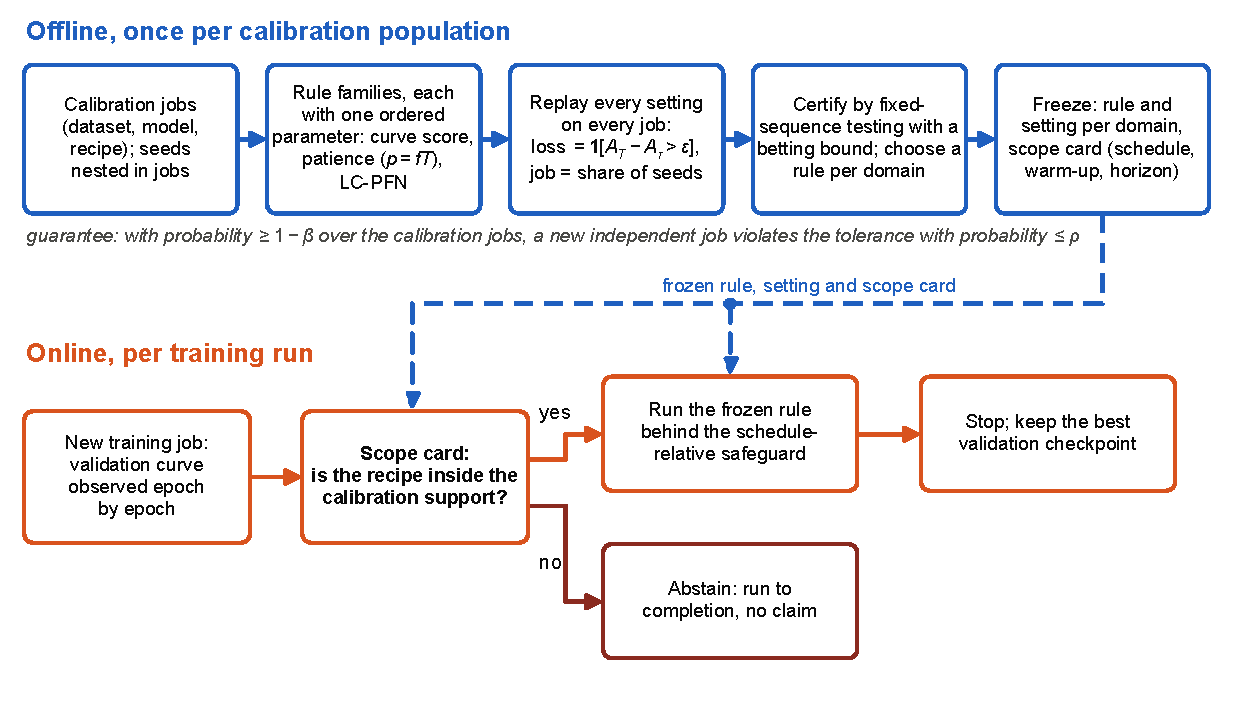
\includegraphics[width=0.85\textwidth]{figures/figure_framework_v3.pdf}
\caption{EcoStop framework. Offline (top): rule families, each with one ordered parameter, are replayed on a calibration population and certified by fixed-sequence testing with a betting bound; the rule and setting per domain are frozen together with a scope card. Online (bottom): a new job inside the scope card runs the frozen rule behind a schedule-relative safeguard and stops; a job outside it abstains and runs to completion.}
\label{fig:framework}
\end{figure*}

\textbf{EcoStop's curve rule.} At epoch $t$ the rule fits the saturation model $Q_\vartheta(u)=a-b\,e^{-cu}$, $\vartheta=(a,b,c)\in[0,a_{\max}]\times[0,200]\times[10^{-4},5]$, to the trailing window $W_t=\{\max(1,t-w+1),\dots,t\}$ ($w=15$, at least four points) by nonlinear least squares,
\begin{equation}
\begin{gathered}
\hat\vartheta_t=\arg\min_{\vartheta}\sum_{u\in W_t}\big(Q_u-Q_\vartheta(u)\big)^2,\\
\hat\Sigma_t=\hat s^2_t\,(J_t^\top J_t)^{-1},
\end{gathered}
\label{eq:fit}
\end{equation}
where $J_t$ is the Jacobian at $\hat\vartheta_t$ and $\hat s^2_t$ the residual variance. With $\bar Q_t=\max_{u\in W_t}Q_u$, the asymptote and its uncertainty are
\begin{equation}
(\hat a_t,\hat\sigma_t)=\begin{cases}
\big(\bar Q_t,\ \sigma^{\mathrm{pin}}_t\big) & \text{if pinned},\\
\big(\max\{\hat a,\bar Q_t\},\ \sigma^{\mathrm{fit}}_t\big) & \text{otherwise},
\end{cases}
\label{eq:asym}
\end{equation}
where the fit is \emph{pinned} when $\hat a\ge a_{\max}-0.5$ (ceiling $a_{\max}=100$), read then as ``converged'' at the window's own maximum, and
\begin{equation}
\begin{gathered}
\sigma^{\mathrm{pin}}_t=\max\{\mathrm{sd}_{u\in W_t}(Q_u),\,0.05\},\\
\sigma^{\mathrm{fit}}_t=\max\{(\hat\Sigma_t)_{aa}^{1/2},\,0.05\}.
\end{gathered}
\label{eq:sigmas}
\end{equation} The predicted remaining gain is $\hat g_t=\hat a_t-B_t$, and, treating it as Gaussian with standard deviation $\hat\sigma_t$, the continuation score is the approximate probability that more than the tolerance remains:
\begin{equation}
s_t=1-\Phi\!\Big(\frac{\epsilon-\hat g_t}{\hat\sigma_t}\Big)\ \approx\ \Pr\big(B_{T_j}-B_t>\epsilon\mid\mathcal{F}_t\big).
\label{eq:score}
\end{equation}
The score need not be calibrated: validity comes from Theorem~\ref{prop:risk}, whatever the quality of the forecast. Two gates guard it. The schedule-relative safeguard requires $t\ge N=\max(2,\mathrm{round}(T_j/8))$; the flat gate requires the best accuracy to have risen by at most $\delta=0.10$\,pp in each of the last $N_f$ epochs,
\begin{equation}
F_t=\mathbf{1}\Big\{\max_{t-N_f<u\le t}(B_u-B_{u-1})\le\delta\Big\}.
\label{eq:flat}
\end{equation}
With $G_t(\gamma)=\mathbf{1}\{t\ge N\}\,\mathbf{1}\{s_t<\gamma\}\,F_t$, the rule with threshold $\gamma$ stops at the first epoch at which the gated signal has held for $k$ consecutive epochs:
\begin{equation}
\tau_\gamma=\min\Big(\Big\{t:\ \textstyle\prod_{u=t-k+1}^{t}G_u(\gamma)=1\Big\}\cup\{T_j\}\Big).
\label{eq:tau}
\end{equation}
The paper rule uses $N_f=N$ and $k=2$; the family is indexed by $\gamma$ on 25 values from 0.02 to 0.98 (larger is more aggressive); constants are in Table~\ref{tab:hyper} and the online procedure in Algorithm~\ref{alg:ecostop}.

\textbf{Schedule-relative variant (EcoStop-SR).} The floors $N_f\ge2$ and $k=2$ are fixed constants. On a 10-epoch fine-tuning run they cap EcoStop at 33.7\% energy-weighted saving whatever $\gamma$ is, because the rule cannot stop before epoch 4. EcoStop-SR uses $N_f=\max(1,\mathrm{round}(T_j/8))$ and $k=\min(2,\max(1,\mathrm{round}(T_j/20)))$; for $T_j\ge30$ it coincides with EcoStop. It was devised after the 142 development jobs had been analysed, which is why \S\ref{sec:c1} tests it on new data.

\begin{lemma}[Monotone stopping]
\label{lem:monotone}
Each $\tau_\gamma$ in \eqref{eq:tau} is a stopping time, and $\gamma\le\gamma'$ implies $\tau_{\gamma'}\le\tau_\gamma$ on every run. Consequently the saving $\Delta_\gamma(j)$ is non-decreasing in $\gamma$ for every job. The same holds for the patience families below as $p$ decreases.
\end{lemma}
\begin{proof}
$G_u(\gamma)$ is a function of $Q_1,\dots,Q_u$, so $\{\tau_\gamma=t\}\in\mathcal{F}_t$. For $\gamma\le\gamma'$, $\mathbf{1}\{s_u<\gamma\}\le\mathbf{1}\{s_u<\gamma'\}$ pointwise, so $G_u(\gamma)\le G_u(\gamma')$ and every epoch that qualifies in \eqref{eq:tau} for $\gamma$ qualifies for $\gamma'$; the minimum over a larger set is smaller. Energy is non-decreasing in $t$, which gives the saving. For patience, the stopping condition $t-\lambda_t\ge p$ in \eqref{eq:pat} is implied by $t-\lambda_t\ge p'$ for $p'\ge p$.
\end{proof}

\noindent The violation $V_\gamma$ is not monotone in $\gamma$, since stopping earlier can keep a checkpoint with higher test accuracy. Lemma~\ref{lem:monotone} orders the family; Theorem~\ref{prop:risk} handles the non-monotone risk.

\textbf{Baselines, all certified identically.} \emph{Patience with minimum improvement $\delta_p$:} with $\lambda_t$ the last epoch $u\le t$ at which $Q_u$ exceeded the previous best by more than $\delta_p$,
\begin{equation}
\tau^{\mathrm{pat}}_{p}=\min\big(\{t: t-\lambda_t\ge p\}\cup\{T_j\}\big),
\label{eq:pat}
\end{equation}
with $p$ fixed in epochs ($p=1,\dots,20$, $\delta_p=0$), or schedule-relative, $p=\max(1,\mathrm{round}(fT_j))$ with $f\in[0.06,0.5]$ and $\delta_p\in\{0,0.1\}$\,pp. \emph{LC-PFN:} the released pretrained network \citep{adriaensen2023lcpfn} gives $s^{\mathrm{PFN}}_t=\Pr_{\mathrm{PFN}}(Q_{T_j}>B_t+\epsilon\mid Q_{1:t})$, used alone ($k=1$, no flat gate; its published rule) or in place of $s_t$ in \eqref{eq:tau}. \emph{Fixed budget fraction:} $\tau_f=\mathrm{round}(f\,T_j)$. We use the original LC-PFN, not a surrogate.


\begin{table*}[t]
\centering
\caption{Rule taxonomy. Every rule is a one-parameter ordered family certified by the same procedure (Table~\ref{tab:symbols} for symbols).}
\label{tab:taxonomy}
\footnotesize
\begin{adjustbox}{max width=\textwidth}
\begin{tabular}{p{3.3cm}p{6.2cm}p{3.0cm}p{2.3cm}}
\toprule
Rule & Components & Free parameter (grid) & Uses $T_j$? \\
\midrule
EcoStop (curve rule) & saturation fit with uncertainty score \eqref{eq:score}; flat gate \eqref{eq:flat}; safeguard $N$; $k{=}2$ consecutive signals & $\gamma$ (25 values) & yes ($N=T_j/8$) \\
EcoStop-SR & as EcoStop with $N_f$ and $k$ scaled to $T_j$ (identical for $T_j\ge30$) & $\gamma$ (25 values) & yes \\
Patience, fixed $p$ & no improvement for $p$ epochs & $p=1,\dots,20$ & no \\
Patience, $p=\lceil fT\rfloor$ (min-$\delta$) & no improvement above $\delta_p$ for $p\propto T_j$ epochs & $f\in[0.06,0.5]$ (12 values) & yes \\
LC-PFN (+ gates) & pretrained extrapolation score; alone ($k{=}1$, no gate) or in the EcoStop gates & $g$ (15 values) & gates only \\
Fixed budget fraction & stop at $\lceil fT\rfloor$ & $f$ (18 values) & yes \\
EcoStop framework & betting certificate; certified rule per domain among the three rules; scope card & shared index $k\le K{=}25$ & yes \\
\bottomrule
\end{tabular}
\end{adjustbox}
\end{table*}

\begin{algorithm}[t]
\caption{EcoStop online rule (deployment of a certified $\hat\gamma$)}
\label{alg:ecostop}
\begin{algorithmic}[1]
\Require recipe with budget $T$ and descriptors $\phi$; scope card $\mathcal{S}$; certified $\hat\gamma$; $\epsilon,\delta,w,N,N_f,k$
\If{$\phi\notin\mathcal{S}$} \State train to $T$; \Return $\kappa_T$ \Comment{abstain (Proposition~\ref{prop:scope})} \EndIf
\State $c\gets0$
\For{$t=1,\dots,T$}
  \State train epoch $t$; observe $Q_t$; $B_t\gets\max(B_{t-1},Q_t)$; update $\kappa_t$
  \If{$t\ge N$ and $|W_t|\ge4$}
    \State fit \eqref{eq:fit}; obtain $(\hat a_t,\hat\sigma_t)$ by \eqref{eq:asym}; $s_t\gets1-\Phi((\epsilon-\hat a_t+B_t)/\hat\sigma_t)$
    \State $G_t\gets\mathbf{1}\{s_t<\hat\gamma\}\cdot F_t$ \Comment{flat gate \eqref{eq:flat}}
    \State $c\gets(c+1)\,G_t$ \Comment{consecutive signals}
    \If{$c\ge k$} \Return $\kappa_t$ \Comment{stop: $\tau=t$} \EndIf
  \Else \State $c\gets0$
  \EndIf
\EndFor
\State \Return $\kappa_T$
\end{algorithmic}
\end{algorithm}

\begin{algorithm}[t]
\caption{Offline certification with rule selection and scope card}
\label{alg:certify}
\begin{algorithmic}[1]
\Require logged calibration jobs $j_1,\dots,j_n$; rules $\mathcal{R}$; domains $\mathcal{D}$; $K$; $\rho$, $\beta$; $p$-value $p(\cdot)$ (Lemma~\ref{lem:hb} or \ref{lem:bet})
\State $\mathcal{A}\gets\mathcal{R}^{\mathcal{D}}$; $C\gets\emptyset$
\For{$a\in\mathcal{A}$}
  \For{$k=1,\dots,K$}
    \State replay $(a,k)$ on every calibration run; $x_l\gets L_{a,k}(j_l)$ \Comment{exact by Lemma~\ref{lem:replay}}
    \If{$p(x_1,\dots,x_n;\rho)\le\beta/|\mathcal{A}|$} \State $C\gets C\cup\{(a,k)\}$ \Else \State \textbf{break} \Comment{fixed sequence \eqref{eq:fixedseq}} \EndIf
  \EndFor
\EndFor
\State $(\hat a,\hat k)\gets\arg\max_{(a,k)\in C}\mathrm{EW}_{\{j_1,\dots,j_n\}}(a,k)$ \Comment{any choice is valid (Theorem~\ref{thm:select})}
\State $\mathcal{S}\gets$ scope card of $\phi(j_1),\dots,\phi(j_n)$ (Definition~\ref{def:scope})
\State \Return $(\hat a,\hat k,\mathcal{S})$, or ``never stop'' if $C=\emptyset$
\end{algorithmic}
\end{algorithm}

\begin{table}[t]
\centering
\caption{Constants of the EcoStop rule and of the evaluation protocol.}
\label{tab:hyper}
\footnotesize
\begin{adjustbox}{max width=\columnwidth}
\begin{tabular}{p{4.3cm}p{3.2cm}}
\toprule
Constant & Value \\
\midrule
Tolerance $\epsilon$ & 0.5\,pp \\
Fit window cap $w$; minimum points & 15; 4 \\
Asymptote ceiling $a_{\max}$ & 100 \\
Safeguard $N$; flat window $N_f$ & $\max(2,\mathrm{round}(T/8))$; $N_f=N$ \\
Flat tolerance $\delta$ & 0.10\,pp \\
Consecutive signals $k$ & 2 \\
Score-threshold grid & 25 values, 0.02 to 0.98 \\
Patience grids & $p=1..20$; $f\in[0.06,0.5]$ \\
Shared selection index $K$ & 25 \\
Risk targets; confidence & $\rho\in\{0.15,0.20\}$ (also 0.10 in RQ6--RQ8); $\beta=0.05$ \\
Cross-fitting & 5 folds $\times$ 20 repeats \\
Random-split test & 1{,}000 splits, 70/30 \\
\bottomrule
\end{tabular}
\end{adjustbox}
\end{table}

\textbf{Overhead.} Replaying the predictor over every logged epoch (23{,}158 scored epochs, 538 runs) cost 259.9\,s of CPU time, 11.2\,ms per scored epoch, against 199{,}300\,s of GPU training: 0.13\% overall (0.02\% vision, 0.004\% NLP, 8.8\% tabular, whose epochs are milliseconds long). As this compares CPU time to GPU time it bounds the controller's energy overhead from above; the energy savings reported below do not subtract it.

\section{Experimental Setup}
\label{sec:setup}

\subsection{Corpus}
\label{sec:corpus}
The development corpus has 142 jobs and 535 runs: 22 vision jobs trained from scratch (ResNet-9/18, SGD, cosine, 40 epochs, 3 seeds), 93 tabular jobs (MLP, 60 epochs, 4--8 seeds) from OpenML \citep{vanschoren2014openml} and scikit-learn, and 27 NLP fine-tuning jobs (DistilBERT \citep{sanh2019distilbert}, 10 epochs, 3 seeds). A further step-decay vision job is used only in the progressive-schedule analysis. Tabular jobs are 65\% of the jobs but a tiny share of energy (mean 82\,J per run against 153\,kJ for vision and 105\,kJ for NLP), so we report both per-job means and \emph{energy-weighted} savings (total joules saved over total joules), which is the quantity a data-centre operator sees.

\textbf{Development corpus.} \emph{Vision:} CIFAR-10, Fashion-MNIST, MNIST, KMNIST, EMNIST (several splits), QMNIST, CIFAR-100, SVHN, GTSRB, Flowers-102, DTD, FGVC-Aircraft, RenderedSST2, Oxford-IIIT Pet, SEMEION, EuroSAT and Imagenette, trained with ResNet-9 or ResNet-18 (SGD, cosine annealing, 40 epochs, 3 seeds). STL-10 and Food-101 were attempted and excluded for wall-clock and download failures unrelated to the method. \emph{Tabular:} Digits, Breast Cancer, Wine and Iris from scikit-learn (8 seeds) and 89 OpenML datasets (4 seeds), cleaned for missing values and categorical encoding; datasets under 60 samples, with a single class, or with exploding one-hot width were excluded. A small MLP is trained for 60 epochs. \emph{NLP:} DistilBERT on 27 tasks with 355 to 120{,}000 training examples and 2 to 151 classes (sentiment, topic and intent tasks, GLUE grammaticality, entailment and paraphrase tasks, TweetEval sub-tasks and stance targets, IMDB, AG News, Yelp and Amazon polarity, CLINC-OOS, SMS Spam), 10 epochs, 3 seeds. Table~\ref{tab:corpus} summarises the development corpus, the fresh test set of \S\ref{sec:b1setup} and the confirmatory study of \S\ref{sec:c1setup}.

\begin{table*}[t]
\centering
\caption{Development corpus, pre-registered fresh test set and confirmatory study (C1; 41 Hugging Face text-classification datasets, listed in the benchmark, two recipes each). Fresh vision datasets: MobileNetV3 on CIFAR-10, Fashion-MNIST, GTSRB, DTD, Flowers-102; ViT-Tiny on CIFAR-10, Fashion-MNIST, KMNIST, Oxford-Pet; ResNet-18 (step) on Fashion-MNIST, DTD, Oxford-Pet, SEMEION; VGG-style on STL-10, RenderedSST2, MNIST. Fresh NLP tasks: Subj, CR, BBC News, hate/offensive speech, student-question categories, BoolQ, SST-5, Enron spam. Fresh tabular: pc4, pendigits, churn, MagicTelescope, hill-valley, gas-drift, nomao, madelon, dna, artificial-characters, collins.}
\label{tab:corpus}
\footnotesize
\begin{adjustbox}{max width=\textwidth}
\begin{tabular}{llrrp{3.4cm}p{3.2cm}r}
\toprule
Set & Domain & Jobs & Runs & Model & Optimiser, schedule & Epochs \\
\midrule
Development & Vision & 22 & 66 & ResNet-9/18 & SGD, cosine & 40 \\
Development & Tabular & 93 & 388 & MLP (64 units) & SGD, cosine & 60 \\
Development & NLP & 27 & 81 & DistilBERT & AdamW, linear warm-up and decay & 10 \\
\midrule
Fresh & Vision, cosine + warm-up & 9 & 27 & MobileNetV3-S (5), ViT-Tiny (4) & AdamW, cosine + warm-up & 50 \\
Fresh & Vision, step decay & 4 & 12 & ResNet-18 & SGD, step decay & 40 \\
Fresh & Vision, one-cycle & 3 & 9 & VGG-style & SGD, one-cycle & 30 \\
Fresh & NLP & 8 & 24 & small BERT (4 layers, 512 units) & AdamW, linear warm-up and decay & 15 \\
Fresh & Tabular & 11 & 44 & MLP (256 units) & AdamW, cosine & 100 \\
\midrule
Confirmatory (C1) & NLP, 8 epochs & 41 & 123 & ELECTRA-small & AdamW, linear warm-up and decay & 8 \\
Confirmatory (C1) & NLP, 12 epochs & 41 & 123 & BERT L6-H512 & AdamW, linear warm-up and decay & 12 \\
\midrule
\multicolumn{2}{l}{Development total} & 142 & 535 & & & \\
\multicolumn{2}{l}{Fresh total} & 35 & 116 & & & \\
\multicolumn{2}{l}{Confirmatory total} & 82 & 246 & & & \\
\bottomrule
\end{tabular}
\end{adjustbox}
\end{table*}

\subsection{Pre-registered fresh test set}
\label{sec:b1setup}
Before any fresh job was trained we froze (i) the method and every threshold calibrated on the 142-job corpus, and (ii) the job registry, in \texttt{b1\_protocol.json} (SHA-256 of the method code and registry, UTC timestamp 2026-10-07T11:44Z); the evaluation script refuses to run if the hashes change. As for the confirmatory study below, the freeze is local and was not deposited in a public registry. Fresh jobs differ from the corpus in architecture, optimiser, schedule and data: MobileNetV3-Small \citep{howard2019mobilenetv3} and a ViT-Tiny \citep{dosovitskiy2021vit} trained with AdamW \citep{loshchilov2019adamw} and cosine schedules with warm-up (50 epochs); ResNet-18 \citep{he2016resnet} with step decay (40 epochs); a VGG-style network with a one-cycle schedule (30 epochs); a small BERT \citep{turc2019wellread} fine-tuned for 15 epochs on eight new text tasks; and a wider MLP trained with AdamW for 100 epochs on 14 OpenML datasets absent from the corpus (three of which the corpus loader cannot split and were dropped before training). Jobs run strictly one at a time so concurrent load cannot contaminate energy readings.

\subsection{Energy measurement}
\label{sec:energy}
Power is sampled from the on-board NVML sensor of an NVIDIA RTX 4080 Laptop GPU every 20\,ms (2\,ms for tabular jobs, whose epochs are padded to a 25\,ms minimum so that at least one sample falls inside each epoch) and integrated trapezoidally per epoch. Reported savings are relative to the same run's own full-training energy. Values are GPU-board energy, not system energy or emissions; the sensor's update interval, idle power and run-to-run repeatability are characterised in \S\ref{sec:rq6b}.

\subsection{Evaluation protocol}
\label{sec:protocol}
Every result on the development corpus is \emph{out-of-fold}: jobs are split into $K{=}5$ folds stratified by domain, each fold is scored with a threshold calibrated on the other four, and the procedure is repeated 20 times with different fold assignments. We also draw 1{,}000 random 70/30 stratified splits to test validity directly, and report job-level bootstrap intervals for paired differences. Targets are $\rho\in\{0.15,0.20\}$ at $\beta=0.05$, $\epsilon=0.5$\,pp; RQ6 to RQ8 add $\rho=0.10$. If nothing is certified in a fold, the run goes to completion (zero savings, zero risk).

\subsection{Confirmatory fine-tuning study (C1)}
\label{sec:c1setup}
C1 tests whether EcoStop's rule beats calibrated patience on short fine-tuning schedules, the regime with the largest remaining headroom: on the development jobs a hindsight oracle saved 75\% of NLP energy (energy-weighted) and the best certified rule about 44\%. The study was specified before any training. We collected 43 English text-classification datasets from the public Hugging Face listing and vetted them only by loading them; two were dropped by fixed size rules (fewer than 2{,}500 training or 800 test rows), leaving 41 datasets, none of which occurs in the development or fresh sets. Each dataset was fine-tuned with two recipes, ELECTRA-small for 8 epochs (learning rate $3\times10^{-4}$) and a 6-layer BERT with 512 hidden units \citep{turc2019wellread} for 12 epochs ($5\times10^{-5}$), both with AdamW, 10\% linear warm-up, linear decay and three seeds, giving 82 jobs and 246 runs. Neither model nor either schedule length occurs in the calibration population. The dataset list, recipes, stopping rules, evaluation code and analysis plan were hashed before training (SHA-256 of the protocol file \texttt{F11AA18D}\dots\texttt{C814EC07}), and the evaluation refuses to run if a hashed file changes. The protocol was frozen by local hashing and was not deposited in a public registry, so its timing rests on our records and file hashes.

The single pre-registered hypothesis (H1) is that EcoStop-SR saves more energy than calibrated schedule-relative patience (with a 0.1\,pp minimum improvement) at a realised job-level risk of at most 0.10. The statistic is the difference of the two rules' best energy-weighted savings at that risk. Inference is a bootstrap over datasets (the two recipes of a dataset move together, 10{,}000 resamples, each rule's operating point re-chosen inside every resample); H1 is supported only if the lower limit of the 95\% interval exceeds zero. Secondary analyses were fixed in the same plan: other risk caps, results per recipe, frozen operating points calibrated on the 177 existing jobs, a per-dataset sign test and sensitivity analyses.

\textbf{Interruptions and deviations.} (i) After 158 of 246 runs the pre-run idle-GPU guard, which waits while GPU utilisation exceeds 10\%, was relaxed to also require board power above 25\,W, because desktop applications held reported utilisation near 19\% at an idle 6\,W and stalled training for 43\,min. This changes only when a run starts. (ii) Windows Modern Standby suspended the machine, once for 12.5\,h. Three finished runs had an epoch whose NVML energy integral spanned a suspension (510\,s to 12.4\,h against a median of 10--12\,s). By an outcome-blind rule written before the evaluation (longest epoch above five times the run median and above 60\,s) they were quarantined and re-run with the same seed; the originals are retained and the rule was re-applied to all runs before evaluation. (iii) The laptop powered off without a clean shutdown four times; training resumed from complete runs only, with the locked files verified before each resumption, and a keep-awake request was added after the standby episode. (iv) An interim look at 69 of 82 jobs was taken at an author's request before the final evaluation; nothing was changed afterwards. (v) The machine was shared with other desktop workloads during part of the study; per-run pre-run GPU state and a 20\,s power and temperature log are kept. (vi) The framework check of \S\ref{sec:c1} was specified after the interim look, so it is a held-out check and not a blind pre-registration.

\subsection{Pooled analysis and regimes}
\label{sec:pooledsetup}
To measure the framework over all the evidence we pool the 142 development, 35 fresh and 82 C1 jobs (259 jobs from 218 datasets: 117 NLP, 104 tabular, 38 vision) and cross-fit it ($K{=}5$ folds, 20 repeats) with folds grouped by dataset, so the two recipes of a C1 dataset never straddle a split, and stratified by domain. The method specification is the one fixed before C1; nothing was tuned on the pooled data. Regimes (domain, architecture, schedule family) are defined after the fact and the intervals are bootstrap intervals over dataset groups: this is an exploratory analysis and not a held-out test, since all of the data had been seen. Validity is checked as coverage over 1{,}000 random 70/30 dataset-grouped splits.

\section{Results}
\label{sec:results}

\subsection{RQ1: Is the certificate valid?}
\label{sec:rq1}
On all 142 jobs, EcoStop's per-run violation risk rises from 0.03 at $\gamma=0.02$ to 0.147 at $\gamma\ge0.58$ and saturates there; the gates, not $\gamma$, then set the stopping time. Calibration at $\beta=0.05$ certifies $\hat\gamma=0.14$ at $\rho=0.15$ and $\hat\gamma=0.46$ at $\rho=0.20$. Out-of-fold, realised risk is 0.071 and 0.115 respectively (Table~\ref{tab:oof}), well below the targets. Over 1{,}000 random 70/30 splits, realised test risk at $\rho=0.20$ exceeded the target on 1.5\% of splits for EcoStop and 1.2\% for calibrated patience (Fig.~\ref{fig:validity}), against the 5\% the guarantee permits. This check is itself conservative in one direction and loose in another: a held-out 30\% sample can exceed $\rho$ through sampling noise even when the population risk does not. We therefore also ran a direct check in which the population is the 142 development jobs, so the true risk of every setting is known exactly: drawing calibration sets of 60, 100 and 142 jobs with replacement 1{,}000 times each, the certified setting's true risk exceeded $\rho$ in at most 0.1\% of draws. The certificate is valid and, as expected of a distribution-free bound, conservative; \S\ref{sec:ext} turns part of that slack into savings.

\begin{figure}[t]
\centering
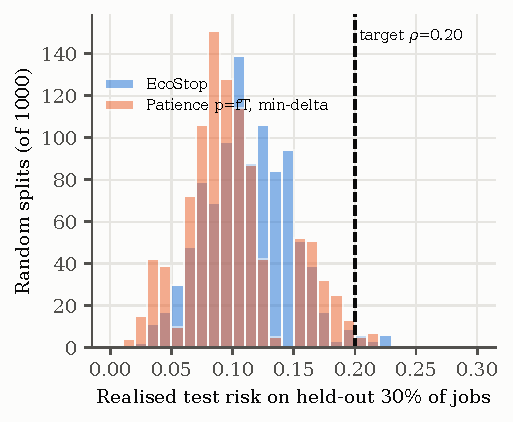
\includegraphics[width=\linewidth]{figures/fig_validity_splits.pdf}
\caption{Realised test risk on the held-out 30\% of jobs over 1{,}000 random calibration/test splits, $\rho=0.20$, $\beta=0.05$. The target is exceeded on 1.5\% (EcoStop) and 1.2\% (patience) of splits.}
\label{fig:validity}
\end{figure}

\subsection{RQ2: Which rule saves most energy at matched risk?}
\label{sec:rq2}
Figure~\ref{fig:frontier} plots out-of-fold risk against savings for every rule as the target $\rho$ varies, and Table~\ref{tab:oof} lists the two operating points. At matched risk, EcoStop, the real LC-PFN under EcoStop's gates, and patience with $p$ proportional to the schedule length and a 0.1\,pp minimum improvement are close: at $\rho=0.20$ they save 50.4\%, 51.7\% and 52.8\% of energy per job and 30.9\%, 30.4\% and 31.8\% energy-weighted. The paired job-bootstrap difference between EcoStop and calibrated patience is $-2.3$\,pp (95\% CI $[-4.9,+0.1]$) at $\rho=0.20$ and $-2.0$\,pp ($[-4.8,+0.7]$) at $\rho=0.15$ (Table~\ref{tab:paired}); we cannot distinguish them.

Two baselines are clearly worse. Patience with a $p$ fixed in epochs saves 44.5--48.9\% per job, comparable to the others, but only 2.9--4.2\% energy-weighted: it cannot fire on 10--15-epoch fine-tuning schedules and fires late on long vision runs, so it forgoes most of the energy. A fixed budget fraction saves 14.9--22.7\% per job and incurs a vision risk of 0.27--0.53, because it cannot adapt to a job's curve. The effect of the schedule is large precisely where it matters: a mean-per-job comparison, which tabular jobs dominate, understates it.

\textbf{Against the defaults in use.} Practitioners rarely calibrate patience; they take the value shipped with a library or a tutorial. Table~\ref{tab:defaults} scores three common values directly, without calibration, on the same development and fresh jobs. A patience of 3 saves the most energy (48.8\% energy-weighted on the development jobs) but loses more than the tolerance on a third of development runs and 46\% of fresh runs, so its savings are bought with the accuracy the user wanted to keep. A patience of 5 is dominated by the certified rule: at $\rho=0.20$ EcoStop saves 30.9\% against 22.0\% with a risk of 0.115 against 0.202 on the development jobs, and 33.1\% against 27.3\% at 0.205 against 0.279 on the fresh jobs. A patience of 10 has the risk of EcoStop at $\rho=0.15$ (0.073 against 0.071) but saves 3.0\% of the energy where the certified rule saves 23.1\%. The certified rules therefore win against the defaults in use, with a stated risk in place of an unknown one; against a patience that is calibrated in the same way they tie.

\begin{table}[t]
\centering
\caption{Common uncalibrated patience defaults versus certified EcoStop. Development figures for EcoStop are out-of-fold; fresh figures use the frozen thresholds. Risk is the probability that a run loses more than 0.5\,pp; EW is the energy-weighted saving (\%).}
\label{tab:defaults}
\footnotesize
\begin{adjustbox}{max width=\columnwidth}
\begin{tabular}{p{3.4cm}rrrr}
\toprule
 & \multicolumn{2}{c}{Development} & \multicolumn{2}{c}{Fresh} \\
\cmidrule(lr){2-3}\cmidrule(lr){4-5}
Rule & Risk & EW & Risk & EW \\
\midrule
Patience $p=3$ & 0.33 & 48.8 & 0.46 & 50.9 \\
Patience $p=5$ & 0.20 & 22.0 & 0.28 & 27.3 \\
Patience $p=10$ & 0.07 & 3.0 & 0.08 & 5.3 \\
EcoStop, certified $\rho=0.15$ & 0.07 & 23.1 & 0.06 & 23.3 \\
EcoStop, certified $\rho=0.20$ & 0.12 & 30.9 & 0.21 & 33.1 \\
\bottomrule
\end{tabular}
\end{adjustbox}
\end{table}

\textbf{Accuracy cost.} Savings are not free, and the risk metric alone does not show how much accuracy is lost. Table~\ref{tab:acc} gives the out-of-fold accuracy gap $A_T-A_\tau$ per job (mean over seeds). At $\rho=0.20$, EcoStop gives up 0.33\,pp of test accuracy on average (90th percentile 1.05\,pp); the retained checkpoint is as good as or better than the fully trained one on 70\% of jobs, and 16\% of jobs lose more than the 0.5\,pp tolerance. At $\rho=0.15$ the mean gap is 0.10\,pp and 8\% of jobs exceed the tolerance. The other schedule-relative rules lose similar amounts (0.34--0.46\,pp at $\rho=0.20$); the fixed budget fraction loses least (0.18\,pp) because it stops so late that it saves little.

\begin{table}[t]
\centering
\caption{Out-of-fold accuracy cost of early stopping (142 jobs, $\beta=0.05$). Gap is $A_T-A_\tau$ in percentage points, averaged over each job's seeds; negative gaps (early checkpoint better on test) count towards ``gap $\le0$''.}
\label{tab:acc}
\footnotesize
\begin{adjustbox}{max width=\columnwidth}
\begin{tabular}{p{3.0cm}rrrr}
\toprule
Rule & \shortstack{Mean\\gap (pp)} & \shortstack{P90\\gap (pp)} & \shortstack{Jobs gap\\$\le0$ (\%)} & \shortstack{Jobs gap\\$>\epsilon$ (\%)} \\
\midrule
\multicolumn{5}{l}{\emph{Target $\rho=0.15$}}\\
EcoStop & +0.10 & 0.37 & 73 & 8 \\
LC-PFN + gates & +0.18 & 0.37 & 77 & 8 \\
Patience $p{=}fT$, min-$\delta$ & +0.12 & 0.40 & 77 & 8 \\
Patience, fixed $p$ & +0.22 & 0.50 & 76 & 11 \\
Fixed budget fraction & +0.08 & 0.29 & 80 & 4 \\
\midrule
\multicolumn{5}{l}{\emph{Target $\rho=0.20$}}\\
EcoStop & +0.33 & 1.05 & 70 & 16 \\
LC-PFN + gates & +0.34 & 0.70 & 67 & 15 \\
Patience $p{=}fT$, min-$\delta$ & +0.44 & 0.69 & 68 & 15 \\
Patience, fixed $p$ & +0.46 & 0.76 & 68 & 15 \\
Fixed budget fraction & +0.18 & 0.60 & 77 & 11 \\
\bottomrule
\end{tabular}
\end{adjustbox}
\end{table}

\begin{figure*}[t]
\centering
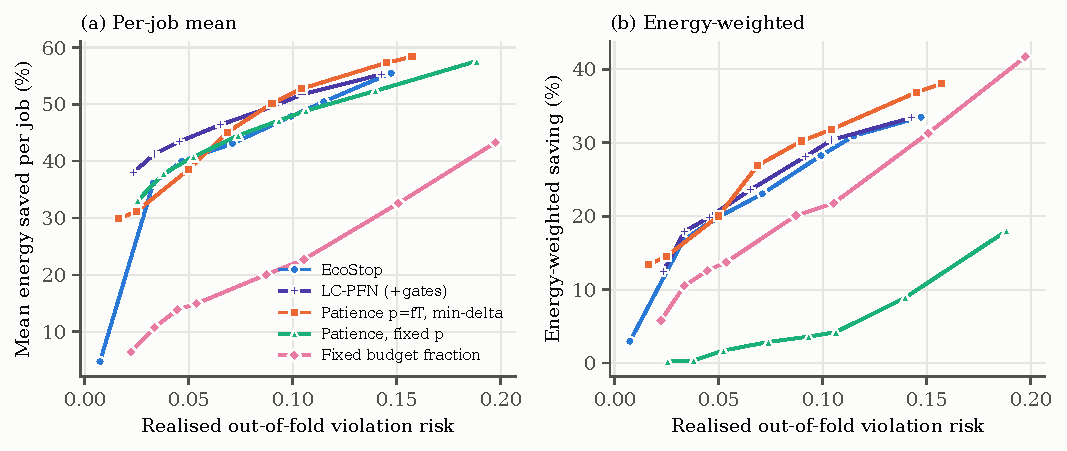
\includegraphics[width=0.85\textwidth]{figures/fig_frontier_oof.pdf}
\caption{Matched-risk comparison. Each point is a target $\rho\in[0.08,0.30]$, $\beta=0.05$; $x$ is the realised out-of-fold risk and $y$ the savings (a: mean per job; b: energy-weighted). Schedule-relative rules (EcoStop, LC-PFN with gates, calibrated patience) coincide within noise; patience fixed in epochs collapses in (b).}
\label{fig:frontier}
\end{figure*}

\begin{table*}[t]
\centering
\caption{Out-of-fold results at matched target risk ($\beta=0.05$, $\epsilon=0.5$\,pp; 142 jobs, 5-fold cross-fitting repeated 20 times). ``Vision risk'' is the realised risk on vision jobs under the pooled threshold; the last column calibrates each domain separately. Best savings per column in bold.}
\label{tab:oof}
\footnotesize
\begin{adjustbox}{max width=\textwidth}
\begin{tabular}{p{4.5cm}rrrrr}
\toprule
Rule & Risk & Vision risk & Mean saved (\%) & Energy-wtd.\ (\%) & Energy-wtd., per-domain (\%) \\
\midrule
\multicolumn{6}{l}{\emph{Target $\rho=0.15$, $\beta=0.05$}}\\
EcoStop (curve score + gates) & 0.07 & 0.16 & 43.1 & 23.1 & 3.6 \\
LC-PFN + EcoStop gates & 0.07 & 0.16 & \textbf{46.4} & 23.6 & 3.3 \\
Patience, $p=\lceil fT\rfloor$, min-$\delta$ & 0.07 & 0.09 & 45.1 & \textbf{26.9} & 7.6 \\
Patience, $p=\lceil fT\rfloor$ & 0.07 & 0.08 & 45.1 & 21.7 & 6.1 \\
Patience, fixed $p$ & 0.07 & 0.08 & 44.5 & 2.9 & 6.1 \\
Fixed budget fraction & 0.05 & 0.27 & 14.9 & 13.8 & 1.8 \\
\midrule
\multicolumn{6}{l}{\emph{Target $\rho=0.20$, $\beta=0.05$}}\\
EcoStop (curve score + gates) & 0.12 & 0.26 & 50.4 & 30.9 & 12.1 \\
LC-PFN + EcoStop gates & 0.10 & 0.24 & 51.7 & 30.4 & 14.5 \\
Patience, $p=\lceil fT\rfloor$, min-$\delta$ & 0.10 & 0.17 & \textbf{52.8} & \textbf{31.8} & 9.4 \\
Patience, $p=\lceil fT\rfloor$ & 0.11 & 0.16 & 52.6 & 25.4 & 7.7 \\
Patience, fixed $p$ & 0.11 & 0.13 & 48.9 & 4.2 & 7.7 \\
Fixed budget fraction & 0.11 & 0.53 & 22.7 & 21.8 & 6.8 \\
\bottomrule
\end{tabular}
\end{adjustbox}
\end{table*}

\begin{table}[t]
\centering
\caption{Paired differences in mean energy saved at matched certified risk (job bootstrap, 5{,}000 resamples).}
\label{tab:paired}
\footnotesize
\begin{adjustbox}{max width=\columnwidth}
\begin{tabular}{lp{3.1cm}rr}
\toprule
$\rho$ & EcoStop minus & \shortstack{$\Delta$ saved\\(pp)} & \shortstack{95\% CI\\(pp)} \\
\midrule
0.15 & Patience $p{=}fT$, min-$\delta$ & -2.0 & [-4.8, +0.7] \\
0.15 & Patience, fixed $p$ & -1.4 & [-4.0, +1.2] \\
0.15 & LC-PFN + gates & -3.3 & [-4.8, -1.7] \\
0.15 & Fixed budget fraction & +28.2 & [+23.8, +32.5] \\
0.20 & Patience $p{=}fT$, min-$\delta$ & -2.3 & [-4.9, +0.1] \\
0.20 & Patience, fixed $p$ & +1.6 & [-0.9, +4.1] \\
0.20 & LC-PFN + gates & -1.3 & [-2.8, +0.1] \\
0.20 & Fixed budget fraction & +27.7 & [+23.4, +31.9] \\
\bottomrule
\end{tabular}
\end{adjustbox}
\end{table}

\subsection{RQ3: Where is the guarantee hard to obtain?}
\label{sec:rq3}
The pooled certificate averages over domains whose risk differs sharply. Under the pooled threshold at $\rho=0.20$, realised risk is 0.26 on vision jobs, against 0.10 on tabular and 0.06 on NLP (Table~\ref{tab:oof}): the 93 tabular jobs dilute vision. Calibrating each domain separately fixes this (vision risk falls to 0.002) but vision is also where energy is concentrated, so energy-weighted savings drop from 30.9\% to 12.1\% for EcoStop and from 31.8\% to 9.4\% for calibrated patience; at $\rho=0.15$ they fall to 3.6\% and 7.6\%, and for EcoStop no threshold at all is certifiable for vision alone on the full corpus. The domains that consume the most energy are the ones where a certificate is hardest and where its price, in forgone savings, is highest. A single pooled number should not be read as a per-domain guarantee.

Table~\ref{tab:domain} gives the domain breakdown under pooled calibration at $\rho=0.20$ (energy-weighted savings are computed within each domain). Rules do not rank the same way in every domain. On NLP, calibrated patience saves more than EcoStop (42.4\% against 18.0\% per job) at a higher risk (0.14 against 0.06): EcoStop is the more conservative rule there. On tabular jobs a patience fixed in epochs does well (72.0\% saved, risk 0.13), because 60-epoch schedules leave it room to fire; its failure is confined to the short NLP schedules (0.8\% saved) and to vision (10.2\%).

\begin{table*}[t]
\centering
\caption{Out-of-fold results by domain under pooled calibration, $\rho=0.20$, $\beta=0.05$. ``Saved'' is the per-job mean energy saved (\%), ``EW'' the energy-weighted saving (\%) within the domain.}
\label{tab:domain}
\footnotesize
\begin{adjustbox}{max width=\textwidth}
\begin{tabular}{p{3.0cm}rrrrrrrrr}
\toprule
 & \multicolumn{3}{c}{Vision} & \multicolumn{3}{c}{NLP} & \multicolumn{3}{c}{Tabular} \\
\cmidrule(lr){2-4}\cmidrule(lr){5-7}\cmidrule(lr){8-10}
Rule & Risk & Saved & EW & Risk & Saved & EW & Risk & Saved & EW \\
\midrule
EcoStop & 0.26 & 24.0 & 32.6 & 0.06 & 18.0 & 31.1 & 0.10 & 66.1 & 61.3 \\
LC-PFN + gates & 0.24 & 23.9 & 31.6 & 0.03 & 20.4 & 30.3 & 0.09 & 67.4 & 60.9 \\
Patience $p{=}fT$, min-$\delta$ & 0.17 & 17.6 & 23.8 & 0.14 & 42.4 & 44.4 & 0.08 & 64.1 & 56.0 \\
Patience, fixed $p$ & 0.13 & 10.2 & 8.9 & 0.00 & 0.8 & 0.3 & 0.13 & 72.0 & 61.3 \\
Fixed budget fraction & 0.53 & 23.0 & 22.5 & 0.02 & 20.6 & 20.3 & 0.03 & 23.3 & 22.9 \\
\bottomrule
\end{tabular}
\end{adjustbox}
\end{table*}

\subsection{RQ4: What makes a rule work?}
\label{sec:ablation}
Table~\ref{tab:ablation} re-fits each variant on the logged trajectories under the same calibration and cross-fitting. Dropping the curve score altogether, leaving only the flat-accuracy gate and the two-signal rule, changes savings by 0.2\,pp (50.6\% vs.\ 50.4\%) per job, lowers energy-weighted savings by 2.1\,pp (28.8\% against 30.9\%) and lowers the realised risk (0.102 against 0.115; vision 0.197 against 0.261). At matched certified risk the learning-curve score therefore does not contribute to the saving, and it accounts for part of EcoStop's higher vision risk (0.261 with it, 0.197 without, against 0.171 for calibrated patience). Replacing the exponential fit with the pretrained LC-PFN changes it by under 2\,pp. Neither the full-history fit, residual-scatter uncertainty, nor removing the bounded-asymptote fallback has a measurable effect on mean savings; the full-history fit costs 6\,pp per job. Two choices matter. The \emph{schedule-relative safeguard} $N=\mathrm{round}(0.125\,T)$: a fixed 5-epoch floor halves energy-weighted savings (16.2\% vs.\ 30.9\%). And \emph{an uncertainty term}: a point-estimate forecast almost never stops (11.1\% per job). Sensitivity to $\epsilon$, window, safeguard fraction, flat tolerance and $k$ is modest (Table~\ref{tab:sens}); savings rise monotonically with $\epsilon$ (55\% at 2\,pp).

\begin{table}[t]
\centering
\caption{Ablation at $\rho=0.20$, $\beta=0.05$, out-of-fold. EW: energy-weighted saving.}
\label{tab:ablation}
\footnotesize
\begin{adjustbox}{max width=\columnwidth}
\begin{tabular}{p{4.6cm}rrrr}
\toprule
Variant & Risk & \shortstack{Vision\\risk} & \shortstack{Mean\\saved (\%)} & \shortstack{EW\\(\%)} \\
\midrule
Full EcoStop & 0.115 & 0.261 & 50.4 & 30.9 \\
No curve score (flat-gate + k only) & 0.102 & 0.197 & 50.6 & 28.8 \\
No flat-gate (score + k only) & 0.102 & 0.240 & 48.1 & 34.8 \\
k=1 (no consecutive-signal rule) & 0.114 & 0.265 & 50.2 & 36.7 \\
Point estimate (no uncertainty) & 0.037 & 0.083 & 11.1 & 8.1 \\
Residual sigma instead of parameter SE & 0.113 & 0.247 & 49.8 & 32.5 \\
Full-history fit (no trailing window) & 0.111 & 0.258 & 44.5 & 31.4 \\
No a_max fallback & 0.112 & 0.248 & 50.3 & 30.0 \\
Fixed 5-epoch safeguard & 0.116 & 0.211 & 47.2 & 16.2 \\
Real LC-PFN: LC-PFN (score only, $k{=}1$) & 0.078 & 0.217 & 49.5 & 27.1 \\
Real LC-PFN: with EcoStop gates & 0.104 & 0.242 & 51.7 & 30.4 \\
\bottomrule
\end{tabular}
\end{adjustbox}
\end{table}

\begin{table}[t]
\centering
\caption{Sensitivity at $\rho=0.20$, $\beta=0.05$, out-of-fold (default: $\epsilon{=}0.5$, $w{=}15$, safeguard 0.125, flat tolerance 0.10, $k{=}2$). EW: energy-weighted saving.}
\label{tab:sens}
\footnotesize
\begin{adjustbox}{max width=\columnwidth}
\begin{tabular}{p{3.6cm}rrr}
\toprule
Setting & Risk & \shortstack{Mean\\saved (\%)} & \shortstack{EW\\(\%)} \\
\midrule
$\epsilon$ (pp) = 0.1 & 0.101 & 43.3 & 22.6 \\
$\epsilon$ (pp) = 0.25 & 0.114 & 48.4 & 28.0 \\
$\epsilon$ (pp) = 1.0 & 0.111 & 54.4 & 33.1 \\
$\epsilon$ (pp) = 2.0 & 0.064 & 55.5 & 33.5 \\
\midrule
window $w$ = 5 & 0.114 & 51.0 & 25.0 \\
window $w$ = 8 & 0.114 & 50.9 & 30.6 \\
window $w$ = 10 & 0.114 & 49.7 & 31.2 \\
window $w$ = 20 & 0.113 & 49.8 & 31.1 \\
\midrule
safeguard fraction = 0.05 & 0.105 & 47.7 & 28.3 \\
safeguard fraction = 0.1 & 0.115 & 48.6 & 28.8 \\
safeguard fraction = 0.2 & 0.080 & 47.7 & 25.8 \\
safeguard fraction = 0.25 & 0.054 & 42.6 & 22.1 \\
\midrule
flat tolerance (pp) = 0.0 & 0.111 & 49.5 & 24.0 \\
flat tolerance (pp) = 0.05 & 0.111 & 50.4 & 28.5 \\
flat tolerance (pp) = 0.2 & 0.115 & 49.6 & 33.8 \\
\midrule
consecutive signals $k$ = 3 & 0.106 & 51.0 & 26.4 \\
consecutive signals $k$ = 4 & 0.080 & 47.6 & 18.2 \\
\bottomrule
\end{tabular}
\end{adjustbox}
\end{table}

\textbf{Tolerance and seed noise.} The violation compares two checkpoints of the \emph{same} run, so differences between runs in absolute accuracy (the SEMEION repeats of \S\ref{sec:rq6b} span 14.5\,pp) do not enter the label directly. Two other sources of noise do: sampling noise of the test set, whose size is the violation rate of the hindsight oracle (7\% on the development jobs and 29\% on fresh vision jobs, \S\ref{sec:b1}), and seed-to-seed variation of the gap itself. Seeds of 66\% of the development jobs differ in final test accuracy by more than the 0.5\,pp tolerance (standard deviation across seeds: median 0.80 for NLP, 1.75 for tabular and 0.24\,pp for vision; 36\% of vision jobs above 0.5\,pp). We therefore re-ran the out-of-fold calibration with a job-specific tolerance $\epsilon_j=\max(0.5,\sigma_{\mathrm{seed},j})$, which raises it for 94 of the 142 jobs. The ranking of the rules is unchanged: calibrated patience saves 30.1\% and 35.9\% energy-weighted at $\rho=0.15$ and $0.20$ against 28.7\% and 33.2\% for the curve rule (with $\epsilon=0.5$: 26.9\% and 31.8\% against 23.1\% and 30.9\%), and realised risks move by at most 0.007 overall. Vision risk rises (curve rule 0.158 to 0.234 at $\rho=0.15$; patience 0.086 to 0.133), so every vision risk in this paper should be read as having a test-noise component that no stopping rule can remove.

\textbf{Unknown horizon (exploratory).} Schedule-relative patience needs the training length $T$ in advance. Open-ended training, such as continual fine-tuning or anytime schedules, has none, and the only calibrated patience available is one fixed in epochs. EcoStop with its original fixed 5-epoch safeguard and 5-epoch flat gate uses no $T$ either. Table~\ref{tab:hf} compares it with fixed-epoch patience at four minimum-improvement settings, all calibrated in the same way. On the development jobs, at matched realised risk, EcoStop saves more energy-weighted than patience with a minimum improvement of 0, 0.1 and 0.2\,pp: $+12.0$ ($[+5.6,+21.0]$), $+6.1$ ($[+2.4,+10.2]$) and $+5.3$\,pp ($[+1.5,+9.2]$) at $\rho=0.20$. It does not beat patience with a minimum improvement of 0.5\,pp, equal to the tolerance ($-0.1$\,pp, $[-9.6,+6.9]$ at $\rho=0.20$; $+2.9$\,pp, $[+0.15,+5.4]$ at $\rho=0.12$). On the 35 fresh jobs, with thresholds calibrated on the development jobs and applied unchanged, all eight comparisons favour EcoStop ($+0.8$ to $+8.2$\,pp at the same target), but only two intervals exclude zero ($+7.5$\,pp against patience with no minimum improvement and $+5.1$\,pp against 0.5\,pp, both at $\rho=0.15$). We regard this as an indication, not a result: the fixed-safeguard variant was the original design constant and its row in the ablation was visible before this comparison, the fresh set is small, and the strongest patience baseline ties. It does suggest that the learning-curve model earns its place when the horizon is unknown, and not when it is known.

\begin{table}[t]
\centering
\caption{Unknown-horizon rules at $\rho=0.20$, $\beta=0.05$. Development: out-of-fold. Fresh: thresholds calibrated on the development jobs and applied unchanged. EW: energy-weighted saving (\%).}
\label{tab:hf}
\footnotesize
\begin{adjustbox}{max width=\columnwidth}
\begin{tabular}{p{3.6cm}rrrr}
\toprule
 & \multicolumn{2}{c}{Development} & \multicolumn{2}{c}{Fresh} \\
\cmidrule(lr){2-3}\cmidrule(lr){4-5}
Rule (no knowledge of $T$) & Risk & EW & Risk & EW \\
\midrule
EcoStop, fixed 5-epoch safeguard & 0.116 & 16.2 & 0.150 & 20.3 \\
Patience, fixed $p$, min-$\delta$ 0 & 0.106 & 4.2 & 0.152 & 12.1 \\
Patience, fixed $p$, min-$\delta$ 0.1 & 0.108 & 10.1 & 0.186 & 16.0 \\
Patience, fixed $p$, min-$\delta$ 0.2 & 0.108 & 10.9 & 0.140 & 13.1 \\
Patience, fixed $p$, min-$\delta$ 0.5 & 0.107 & 16.3 & 0.167 & 19.5 \\
\bottomrule
\end{tabular}
\end{adjustbox}
\end{table}

\subsection{RQ5: Does the certificate survive a shift in architecture, optimiser and schedule?}
\label{sec:b1}
We applied the thresholds frozen before training (\S\ref{sec:b1setup}) to 35 fresh jobs (116 runs: 16 vision, 8 NLP, 11 tabular), without any re-tuning. Table~\ref{tab:b1} gives the realised per-run risk, Fig.~\ref{fig:b1risk} summarises it for EcoStop by domain, and Table~\ref{tab:b1sched} splits vision by schedule family.

\begin{figure}[t]
\centering
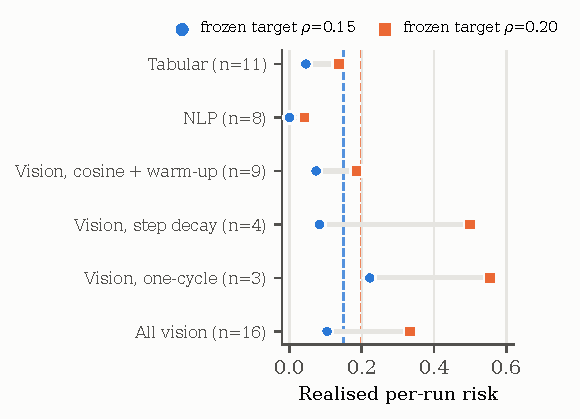
\includegraphics[width=\linewidth]{figures/fig_b1_fresh_risk.pdf}
\caption{Realised per-run violation risk of EcoStop on the 35 fresh jobs, with thresholds frozen before training, by domain and (for vision) by schedule family. Dashed lines mark the two targets. NLP and tabular jobs and cosine-style vision jobs stay near or under the targets; step-decay and one-cycle vision jobs, absent from calibration, do not at $\rho=0.20$.}
\label{fig:b1risk}
\end{figure}

\textbf{At $\rho=0.15$ the pooled certificate transfers.} EcoStop's realised risk is 0.062 (95\% job-bootstrap CI $[0.017,0.114]$), with 0.104 on vision, 0.000 on NLP and 0.045 on tabular jobs, all below the target. The rule saves 37.4\% of energy per job and 23.3\% energy-weighted, close to the 43.1\% and 23.1\% measured out-of-fold on the development corpus.

\textbf{At $\rho=0.20$ it transfers for NLP and tabular jobs but not for vision.} Overall risk is 0.205 ($[0.105,0.312]$), on the target, but the vision component is 0.333, against 0.042 for NLP and 0.136 for tabular. The two language-and-tabular domains, which changed model (a small BERT instead of DistilBERT), schedule length (15 instead of 10 epochs), optimiser and, for tabular, MLP width and epochs, stay within the target. Calibrated patience behaves the same way (overall 0.214, vision 0.417).

\textbf{The vision failure is a schedule-family effect.} Fresh vision jobs under cosine annealing with warm-up (MobileNetV3, ViT-Tiny; 9 jobs), the family closest to the calibration schedules, have risk 0.19 for EcoStop and 0.15 for calibrated patience, within the 0.20 target. Jobs under step decay (ResNet-18; 4 jobs) and one-cycle (VGG-style; 3 jobs), schedules absent from the calibration pool (the corpus has a single step-decay job, held out of calibration, and no one-cycle job), have risk 0.50 and 0.56 for EcoStop (0.75 and 0.78 for patience). Both schedules produce long plateaus followed by sudden gains after a learning-rate drop, which a rule that stops on a plateau mistakes for convergence; Fashion-MNIST under step decay and MNIST under one-cycle each violate on all three seeds while saving 58\% and 73\% of energy (Fig.~\ref{fig:traj}). Two further observations qualify these numbers. (i) Two MobileNetV3 jobs (DTD and Flowers-102) never left chance accuracy (2.2\% and 1.0\% best validation accuracy); stopping them saves 85\% of energy at no loss, which flatters the savings. Excluding them raises EcoStop's vision risk to 0.38 and lowers its vision savings from 33.8\% to 26.5\% (Table~\ref{tab:b1sched}). We kept them in Table~\ref{tab:b1}, as the protocol had no exclusion rule. (ii) The hindsight oracle itself violates the 0.5\,pp tolerance on 29\% of fresh vision jobs (7\% on the development corpus), because on small test sets validation-selected and test-selected checkpoints differ by more than the tolerance. Part of the vision risk is therefore test-set noise that no stopping rule can remove.

\textbf{Reading.} Theorem~\ref{prop:risk} concerns jobs drawn from the calibration population (Assumption~\ref{ass:iid}). Fresh step-decay and one-cycle vision jobs are outside it, and the failure marks the edge of the certificate rather than a flaw in the test: a rule calibrated mostly on cosine schedules should be re-calibrated when the schedule family changes. Two safeguards help in practice: the more conservative target ($\rho=0.15$) kept vision within bounds, and domain-conditional calibration, which for EcoStop certifies no vision threshold at all, would have refused to stop vision runs rather than over-stop them (per-domain risk 0.05 overall, 0.00 on vision, at 14.0\% energy-weighted savings).

\begin{table*}[t]
\centering
\caption{Frozen-protocol results on the 35 fresh jobs (116 runs). Thresholds were fixed before any fresh job was trained; risk is the per-run violation probability with a 95\% job-bootstrap interval; ``per-domain EW'' uses domain-conditional thresholds. Savings are relative to each run's own full-training energy.}
\label{tab:b1}
\footnotesize
\begin{adjustbox}{max width=\textwidth}
\begin{tabular}{p{3.6cm}rrrrrrr}
\toprule
Rule & Risk [95\% CI] & Vision & NLP & Tabular & Mean saved (\%) & Energy-wtd. (\%) & Per-domain EW (\%) \\
\midrule
\multicolumn{8}{l}{\emph{Frozen target $\rho=0.15$, $\beta=0.05$}}\\
EcoStop (curve score + gates) & 0.06 [0.02, 0.11] & 0.10 & 0.00 & 0.05 & 37.4 & 23.3 & 12.1 \\
LC-PFN + EcoStop gates & 0.09 [0.02, 0.17] & 0.15 & 0.00 & 0.07 & 35.1 & 22.9 & 12.6 \\
Patience, $p=\lceil fT\rfloor$, min-$\delta$ & 0.05 [0.00, 0.12] & 0.08 & 0.04 & 0.00 & 30.4 & 17.1 & 5.3 \\
Patience, $p=\lceil fT\rfloor$ & 0.05 [0.00, 0.11] & 0.08 & 0.04 & 0.00 & 29.3 & 15.0 & 3.8 \\
Patience, fixed $p$ & 0.08 [0.02, 0.15] & 0.04 & 0.00 & 0.18 & 30.6 & 5.3 & 10.3 \\
Fixed budget fraction & 0.15 [0.07, 0.25] & 0.25 & 0.00 & 0.11 & 19.6 & 19.8 & 4.3 \\
\midrule
\multicolumn{8}{l}{\emph{Frozen target $\rho=0.20$, $\beta=0.05$}}\\
EcoStop (curve score + gates) & 0.21 [0.11, 0.31] & 0.33 & 0.04 & 0.14 & 47.3 & 33.1 & 14.0 \\
LC-PFN + EcoStop gates & 0.15 [0.06, 0.26] & 0.25 & 0.04 & 0.09 & 41.1 & 29.0 & 16.2 \\
Patience, $p=\lceil fT\rfloor$, min-$\delta$ & 0.21 [0.11, 0.32] & 0.42 & 0.04 & 0.05 & 46.5 & 34.0 & 7.8 \\
Patience, $p=\lceil fT\rfloor$ & 0.16 [0.08, 0.24] & 0.29 & 0.04 & 0.05 & 41.8 & 27.0 & 7.6 \\
Patience, fixed $p$ & 0.15 [0.07, 0.25] & 0.21 & 0.00 & 0.18 & 37.4 & 12.1 & 13.0 \\
Fixed budget fraction & 0.25 [0.12, 0.38] & 0.44 & 0.04 & 0.11 & 24.5 & 24.6 & 8.4 \\
\bottomrule
\end{tabular}
\end{adjustbox}
\end{table*}

\begin{table}[t]
\centering
\caption{Fresh vision jobs by schedule family at the frozen $\rho=0.20$ thresholds. ``Oracle risk'' is the violation rate of the hindsight oracle, a test-noise floor. The last row excludes two jobs that never left chance accuracy. Eco: EcoStop; Pat.: calibrated patience with $p$ proportional to $T$ and a minimum improvement.}
\label{tab:b1sched}
\footnotesize
\begin{adjustbox}{max width=\columnwidth}
\begin{tabular}{p{2.6cm}rrrrrr}
\toprule
Schedule family & Jobs & \shortstack{Eco\\risk} & \shortstack{Eco\\saved (\%)} & \shortstack{Pat.\\risk} & \shortstack{Pat.\\saved (\%)} & \shortstack{Oracle\\risk} \\
\midrule
cosine + warm-up & 9 & 0.19 & 30.6 & 0.15 & 27.8 & 0.30 \\
step decay & 4 & 0.50 & 32.8 & 0.75 & 42.1 & 0.33 \\
one-cycle & 3 & 0.56 & 44.9 & 0.78 & 56.0 & 0.22 \\
all vision & 16 & 0.33 & 33.8 & 0.42 & 36.6 & 0.29 \\
all vision, excl. non-learning & 14 & 0.38 & 26.5 & 0.48 & 30.2 & -- \\
\bottomrule
\end{tabular}
\end{adjustbox}
\end{table}

\textbf{Scope card and abstention.} The failure above is a scope violation, and a certificate can say so itself. We attach to each certificate the support of its calibration population in four recipe descriptors: the largest sudden learning-rate drop (at least 50\% from one epoch to the next, before 90\% of the horizon), the warm-up fraction, the horizon (within a factor of two of the calibration range of the domain), and the domain. A job whose declared recipe falls outside the card abstains: it runs to completion, with zero savings and zero risk. Computed on the 142 development jobs, the card admits sudden drops below 0.4, warm-up fractions up to 0.10, and horizons of 10, 40 and 60 epochs for NLP, vision and tabular jobs. Applied to the 35 fresh jobs it flags exactly the 7 step-decay and one-cycle jobs (the step-decay ones by their 90\% drop, the one-cycle ones by their 30\% warm-up fraction) and keeps the cosine-with-warm-up, NLP and tabular jobs in scope. With the frozen thresholds at $\rho=0.20$, abstention lowers EcoStop's risk from 0.205 to 0.100 and calibrated patience's from 0.214 to 0.062, and the vision risk from 0.33 and 0.42 to 0.10 and 0.08 (Table~\ref{tab:scope}). The risk on the in-scope jobs alone is 0.125 and 0.077. The price is the savings forgone on the abstained jobs, 11\,pp energy-weighted for EcoStop (33.1\% to 22.0\%) and 12\,pp for patience, much of which was obtained by violating the tolerance. The descriptors were chosen after we had seen which fresh jobs failed, so this result shows that the mechanism works, not that these four descriptors are sufficient; a confirmatory set is needed.

\begin{table}[t]
\centering
\caption{Scope-card abstention on the 35 fresh jobs at the frozen $\rho=0.20$ thresholds. ``Vision'' is the risk on the 16 fresh vision jobs; EW is the energy-weighted saving. The card abstains on 7 jobs.}
\label{tab:scope}
\footnotesize
\begin{adjustbox}{max width=\columnwidth}
\begin{tabular}{p{2.5cm}lrrr}
\toprule
Rule & Policy & Risk & Vision & EW (\%) \\
\midrule
EcoStop & every job & 0.21 & 0.33 & 33.1 \\
 & scope card & 0.10 & 0.10 & 22.0 \\
Patience $p{=}fT$, min-$\delta$ & every job & 0.21 & 0.42 & 34.0 \\
 & scope card & 0.06 & 0.08 & 21.9 \\
Patience, fixed $p$ & every job & 0.15 & 0.21 & 12.1 \\
 & scope card & 0.08 & 0.04 & 6.8 \\
\bottomrule
\end{tabular}
\end{adjustbox}
\end{table}

\begin{figure*}[t]
\centering
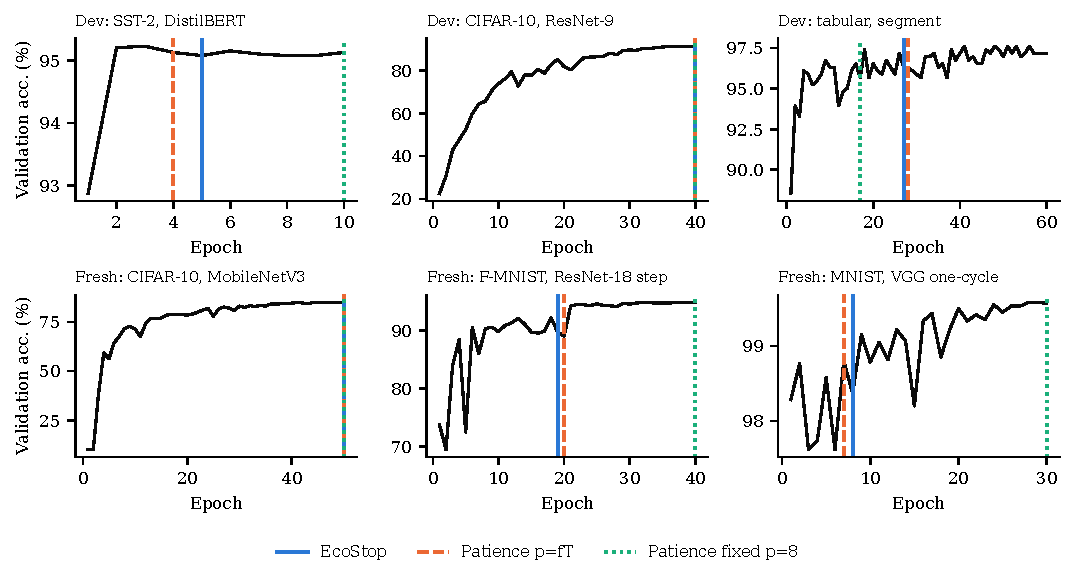
\includegraphics[width=0.9\textwidth]{figures/fig_trajectories.pdf}
\caption{Example validation curves (seed 0) with the stopping epoch of each frozen rule at $\rho=0.20$. Top: development jobs, where rules stop on a genuine plateau (SST-2, tabular) or run to the end because the curve never plateaus (CIFAR-10, ResNet-9). Bottom: fresh jobs. Under cosine annealing with warm-up the rules behave as on the development jobs; under step decay (Fashion-MNIST) and one-cycle (MNIST) both schedule-relative rules stop on a plateau just before accuracy jumps after the learning-rate drop, which is the failure behind the vision risk in Table~\ref{tab:b1sched}.}
\label{fig:traj}
\end{figure*}

\subsection{Framework extensions and the full framework against standard certification}
\label{sec:ext}
Both extensions of \S\ref{sec:problem} reuse the logged runs; nothing was retrained.

\textbf{Betting certificate.} On the development jobs, out-of-fold with the same folds, the betting certificate raises the energy-weighted saving of every rule at the same target: at $\rho=0.15$ from 23.5\% to 28.2\% for EcoStop, 27.1\% to 29.7\% for calibrated patience and 23.8\% to 27.6\% for LC-PFN with gates; at $\rho=0.20$ by 1.6--2.9\,pp. It does so by spending the slack the Hoeffding--Bentkus certificate leaves: in the known-true-risk check of \S\ref{sec:rq1} the certified setting's true risk exceeded $\rho$ in at most 2.7\% of draws (5\% permitted), and the true risk of the chosen setting moved closer to the target (EcoStop at $\rho=0.20$, $n=142$: 0.136 against 0.122). The slack also protected against shift. Calibrated on the development jobs and applied to all 35 fresh jobs, the tighter certificate lets EcoStop exceed its target at $\rho=0.15$ (0.167). Combined with the scope card, it does not: the risk on in-scope fresh jobs is 0.101 for EcoStop and 0.036 for calibrated patience, and the energy-weighted saving with abstention rises from 18.9\% to 21.3\% and from 14.7\% to 19.9\% compared with the Hoeffding--Bentkus certificate with the same scope card. A tighter certificate and a scope card belong together.

\textbf{Certified rule selection.} No single rule is best everywhere (Table~\ref{tab:domain}). With EcoStop, calibrated patience and LC-PFN with gates as candidates (27 assignments, betting certificate), certified selection beats every single rule at matched realised risk on the development jobs, out-of-fold: by 5.3\,pp ($[+1.9,+9.0]$) against calibrated patience, 9.9\,pp ($[+6.0,+14.2]$) against EcoStop and 6.5\,pp ($[+3.1,+9.9]$) against LC-PFN at a risk near 0.10, and in all nine comparisons across risk levels the interval excludes zero (Table~\ref{tab:portfolio}). It chooses patience for NLP, LC-PFN for tabular jobs and EcoStop (at $\rho=0.20$) or LC-PFN (at $\rho=0.15$) for vision, and its true-risk validity check exceeds $\rho$ in at most 0.1\% of draws. The advantage does not survive the shift to the fresh jobs: calibrated on the development jobs and applied unchanged, it ties the single rules at matched realised risk (27.5\% against 26.3--27.8\% at a risk of 0.12; 31.0\% against 29.1--29.8\% at 0.15). The selection exploits the structure of the calibration population, for example that patience suits the 10-epoch DistilBERT jobs, and that structure did not carry over to new models and recipes. Rule selection is worth doing within a population and should be repeated when the population changes.

\textbf{The full framework against standard certification.} We define the EcoStop framework as the three parts together (the betting certificate, certified per-domain selection over the three rules, and the scope card) and compare it with what a practitioner would assemble from the literature: Learn-then-Test with a Hoeffding--Bentkus p-value, applied to one rule, at the same target $\rho$ and confidence. Two risk-control procedures with the same guarantee are compared by what they deliver at that guarantee, as conformal methods are compared by set size at the same coverage. We fixed this comparison, its three targets and its primary baseline (calibrated patience, the strongest single rule) before running it. It was specified after its components had been examined, including on the fresh jobs, so the fresh panel is a held-out check of the combination, not a pre-registered test. On the development jobs, out-of-fold, the framework saves more energy than every baseline at $\rho=0.15$ and $0.20$, by 4.4--8.0\,pp with all six intervals above zero, at a lower realised risk (Table~\ref{tab:pipeline}). At $\rho=0.10$ the Bonferroni correction over 27 assignments costs power and the intervals include zero. On the fresh jobs, where every baseline is also given the scope card, eight of nine differences favour the framework; the primary comparison at $\rho=0.20$ excludes zero ($+2.1$\,pp, $[+0.1,+5.6]$), as does the comparison with LC-PFN ($+4.3$\,pp, $[+0.7,+10.5]$). Its realised risk stays within every target (at most 0.079), whereas standard certification without the scope card reaches 0.214 at $\rho=0.20$. With 35 fresh jobs the intervals are wide; the development result is the firm one.

\begin{table*}[t]
\centering
\caption{The full EcoStop framework (betting certificate, certified per-domain rule selection, scope card) against standard Learn-then-Test certification (LTT-HB: Hoeffding--Bentkus p-value, one rule) at the same target $\rho$, $\beta=0.05$. EW: energy-weighted saving (\%); Risk: realised risk. Development: out-of-fold (5 folds $\times$ 20 repeats). Fresh: calibrated on the development jobs and applied unchanged; every method, baselines included, abstains outside the scope card. Last row of each panel: framework minus the strongest baseline (calibrated patience) in pp, with a paired job-bootstrap 95\% interval.}
\label{tab:pipeline}
\footnotesize
\begin{adjustbox}{max width=\textwidth}
\begin{tabular}{lrrrrrr}
\toprule
 & \multicolumn{2}{c}{$\rho=0.10$} & \multicolumn{2}{c}{$\rho=0.15$} & \multicolumn{2}{c}{$\rho=0.20$} \\
\cmidrule(lr){2-3}\cmidrule(lr){4-5}\cmidrule(lr){6-7}
Method & EW & Risk & EW & Risk & EW & Risk \\
\midrule
\multicolumn{7}{l}{\emph{Development jobs (142), out-of-fold}}\\
LTT-HB, curve rule & 16.9 & 0.03 & 23.5 & 0.07 & 30.9 & 0.11 \\
LTT-HB, calibrated patience & 14.3 & 0.03 & 27.1 & 0.07 & 32.0 & 0.11 \\
LTT-HB, LC-PFN + gates & 18.2 & 0.03 & 23.8 & 0.07 & 30.4 & 0.10 \\
EcoStop framework & \textbf{19.8} & 0.03 & \textbf{31.5} & 0.06 & \textbf{37.2} & 0.10 \\
Framework $-$ patience & \multicolumn{2}{c}{$+5.6$ $[-0.1,+12.8]$} & \multicolumn{2}{c}{$+4.4$ $[+1.4,+7.7]$} & \multicolumn{2}{c}{$+5.2$ $[+2.0,+9.0]$} \\
\midrule
\multicolumn{7}{l}{\emph{Fresh jobs (35), calibrated on development, scope card for every method}}\\
LTT-HB, curve rule & 15.8 & 0.00 & \textbf{18.9} & 0.03 & 22.0 & 0.10 \\
LTT-HB, calibrated patience & 7.9 & 0.00 & 14.7 & 0.01 & 21.9 & 0.06 \\
LTT-HB, LC-PFN + gates & 12.2 & 0.02 & 17.1 & 0.04 & 19.7 & 0.06 \\
EcoStop framework & \textbf{16.5} & 0.03 & 18.5 & 0.04 & \textbf{24.0} & 0.08 \\
Framework $-$ patience & \multicolumn{2}{c}{$+8.6$ $[-1.4,+18.6]$} & \multicolumn{2}{c}{$+3.8$ $[-2.8,+9.0]$} & \multicolumn{2}{c}{$+2.1$ $[+0.1,+5.6]$} \\
\bottomrule
\end{tabular}
\end{adjustbox}
\end{table*}

\begin{table}[t]
\centering
\caption{Certified rule selection against single rules, energy-weighted saving (\%) at matched realised risk. All rules use the betting certificate. Development: out-of-fold. Fresh: calibrated on the development jobs and applied unchanged.}
\label{tab:portfolio}
\footnotesize
\begin{adjustbox}{max width=\columnwidth}
\begin{tabular}{p{2.8cm}rrrr}
\toprule
 & \multicolumn{2}{c}{Development, risk} & \multicolumn{2}{c}{Fresh, risk} \\
\cmidrule(lr){2-3}\cmidrule(lr){4-5}
Rule & 0.08 & 0.10 & 0.12 & 0.15 \\
\midrule
EcoStop & 25.3 & 28.3 & 27.3 & 29.3 \\
Patience $p{=}fT$, min-$\delta$ & 29.1 & 31.3 & 27.8 & 29.8 \\
LC-PFN + gates & 26.3 & 29.8 & 26.3 & 29.1 \\
Certified selection & \textbf{34.2} & \textbf{37.3} & 27.5 & 31.0 \\
\bottomrule
\end{tabular}
\end{adjustbox}
\end{table}

\subsection{RQ6: Does the framework beat standard certification, and where?}
\label{sec:regime}
\textbf{Pooled out-of-fold.} Table~\ref{tab:pooled} and Fig.~\ref{fig:pooled} compare the framework with standard certification (Hoeffding--Bentkus, one rule) and with the betting certificate alone. At each target the framework saves more energy than every single-rule standard certificate, by 3.8 to 6.8\,pp; eight of nine intervals exclude zero, the exception being LC-PFN at $\rho=0.15$ ($+4.0$, $[-1.0,+8.6]$). Against the betting certificate alone, which isolates what rule selection adds, the margin is 1.6 to 5.0\,pp; the interval excludes zero for all three rules at $\rho=0.20$ and for the curve rule at $\rho=0.10$ ($+1.9$, $[+0.5,+3.4]$). Over 1{,}000 random dataset-grouped splits the framework's realised risk exceeded $\rho$ in 1.6\% ($\rho=0.15$) and 1.2\% ($\rho=0.20$) of splits, against the 5\% permitted. For the betting certificate on a single rule the same check exceeded $\rho$ in 8.5\% (curve rule) and 7.0\% (LC-PFN) of splits at $\rho=0.15$ and 4.8\% (patience) at $\rho=0.20$. This check counts sampling noise in the held-out 30\% as well as population risk, and the known-true-risk check of \S\ref{sec:ext} found at most 2.7\%, so it does not show the betting certificate to be invalid; it does show that it leaves little margin on held-out data, and that the Bonferroni correction of the selection step restores one. The pooled analysis does not apply the scope card: every job, including the seven fresh step-decay and one-cycle jobs, is stopped.

\begin{table}[t]
\centering
\caption{Pooled out-of-fold results on 259 jobs (218 dataset groups), same target $\rho$ and $\beta=0.05$ for every method. EW: energy-weighted saving (\%); risk: realised per-run violation probability. LTT-HB: Hoeffding--Bentkus fixed-sequence certification of one rule; betting: the betting certificate of \S\ref{sec:ext} for one rule; framework: betting certificate with certified per-domain selection among the three rules (the scope card is not applied here). Last row: framework minus the best LTT-HB single rule (pp, 95\% bootstrap interval over datasets).}
\label{tab:pooled}
\footnotesize
\begin{adjustbox}{max width=\columnwidth}
\begin{tabular}{lrrrrrr}
\toprule
 & \multicolumn{2}{c}{$\rho=0.10$} & \multicolumn{2}{c}{$\rho=0.15$} & \multicolumn{2}{c}{$\rho=0.20$} \\
\cmidrule(lr){2-3}\cmidrule(lr){4-5}\cmidrule(lr){6-7}
Method & EW & Risk & EW & Risk & EW & Risk \\
\midrule
LTT-HB, curve rule & 21.9 & 0.05 & 28.2 & 0.10 & 33.5 & 0.13 \\
LTT-HB, calibrated patience & 20.2 & 0.05 & 29.6 & 0.09 & 32.0 & 0.10 \\
LTT-HB, LC-PFN + gates & 21.8 & 0.05 & 29.4 & 0.09 & 33.5 & 0.13 \\
Betting, curve rule & 25.2 & 0.07 & 30.4 & 0.11 & 33.6 & 0.13 \\
Betting, calibrated patience & 23.3 & 0.06 & 31.8 & 0.10 & 33.5 & 0.12 \\
Betting, LC-PFN + gates & 24.6 & 0.06 & 31.2 & 0.10 & 33.5 & 0.13 \\
EcoStop framework & \textbf{27.0} & 0.05 & \textbf{33.3} & 0.09 & \textbf{38.4} & 0.12 \\
\midrule
Framework $-$ best LTT-HB & \multicolumn{2}{c}{$+5.1$ $[+2.8,+7.8]$} & \multicolumn{2}{c}{$+3.8$ $[+1.5,+6.1]$} & \multicolumn{2}{c}{$+4.9$ $[+3.0,+7.0]$} \\
\bottomrule
\end{tabular}
\end{adjustbox}
\end{table}

\begin{figure}[t]
\centering
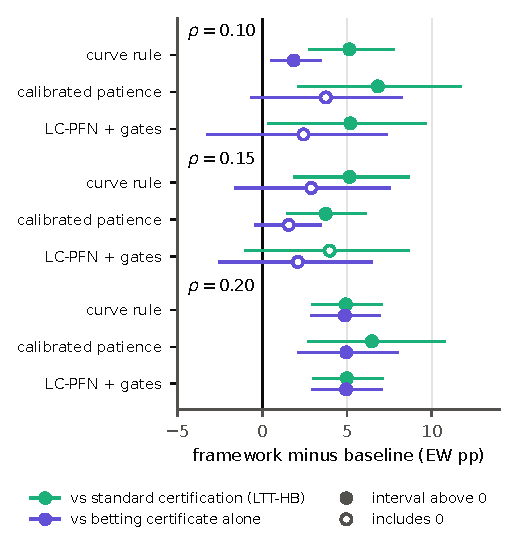
\includegraphics[width=\linewidth]{figures/fig_pooled.pdf}
\caption{The framework against standard certification, pooled out-of-fold over 259 jobs: energy-weighted saving of the framework minus that of a single rule, at the same target $\rho$ and $\beta=0.05$, with 95\% bootstrap intervals over datasets. Green: against standard Learn-then-Test certification (Hoeffding--Bentkus); violet: against the betting certificate alone, which isolates what rule selection adds. Filled marker: interval above zero; hollow: includes zero. Same data as Table~\ref{tab:pooled}.}
\label{fig:pooled}
\end{figure}

\textbf{Regimes.} Table~\ref{tab:regime} and Fig.~\ref{fig:regime} break the comparison with calibrated patience down by domain. In vision (38 jobs, 49\% of the energy) the framework saves 7.1 and 13.5\,pp more at $\rho=0.15$ and $0.20$, and in tabular training (104 jobs, 0.2\% of the energy) 8.0 and 6.9\,pp. In NLP fine-tuning (117 jobs, 51\% of the energy) the framework is within 1\,pp of calibrated patience ($+0.9$ and $-0.3$), because selection chooses patience there. EcoStop's curve rule alone saves 11.7 and 14.1\,pp more than patience in vision and 12.6 and 10.2\,pp in tabular training, but loses 13.7 and 10.4\,pp in NLP; DistilBERT, ELECTRA-small and the 6-layer BERT behave alike. The pooled rule comparison of \S\ref{sec:rq2} is a tie because these gains and losses cancel. The vision row includes the seven fresh step-decay and one-cycle jobs; restricted to the 126 cosine-annealed jobs (development vision and all tabular jobs) the framework's margin is $+7.5$ ($[+3.9,+11.1]$) and $+13.9$\,pp ($[+7.2,+19.7]$), and on the nine fresh cosine-with-warm-up vision jobs it is $+1.9$ ($[-13.4,+11.5]$) and $+8.9$\,pp ($[+0.8,+19.8]$).

\begin{figure*}[t]
\centering
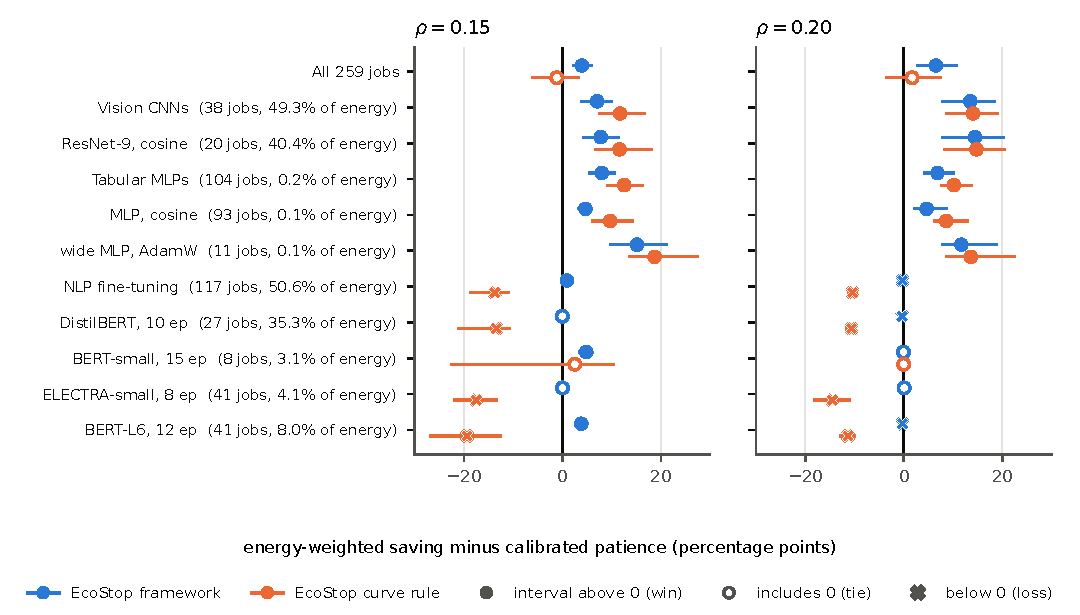
\includegraphics[width=0.92\textwidth]{figures/fig_regime.pdf}
\caption{Where EcoStop wins. Energy-weighted saving minus calibrated patience, both certified with the Hoeffding--Bentkus bound at the same $\rho$, pooled out-of-fold over 259 jobs, with 95\% bootstrap intervals over datasets. Blue: the EcoStop framework; orange: EcoStop's curve rule alone. Filled marker: interval above zero; hollow: includes zero; cross: below zero (the crosses at about $-0.3$\,pp for the framework in NLP at $\rho=0.20$ are statistically below zero but negligible). Subgroups are defined after the fact; step-decay and one-cycle jobs (fewer than six each) have no row of their own but are included in the vision row. Fold assignments differ from those of Table~\ref{tab:pooled}, hence small differences (e.g. $+4.0$ against $+3.8$\,pp for all jobs at $\rho=0.15$).}
\label{fig:regime}
\end{figure*}

\begin{table*}[t]
\centering
\caption{Regimes at $\rho=0.15$ and $\rho=0.20$ (pooled out-of-fold, 259 jobs). EW: energy-weighted saving (\%) within the domain; differences are against LTT-HB calibrated patience (pp, 95\% bootstrap interval over datasets). ``Risk'' is the realised per-run violation probability within the domain: the guarantee is pooled, so a domain can exceed $\rho$ while the pool does not. The vision row includes the seven fresh step-decay and one-cycle jobs; the scope card is not applied in the pooled analysis.}
\label{tab:regime}
\footnotesize
\begin{adjustbox}{max width=\textwidth}
\begin{tabular}{lrrrrrllrr}
\toprule
 & & & \multicolumn{2}{c}{EW} & \multicolumn{2}{c}{Difference from patience} & & \multicolumn{2}{c}{Risk} \\
\cmidrule(lr){4-5}\cmidrule(lr){6-7}\cmidrule(lr){9-10}
Domain & Jobs & Energy (\%) & Framework & Patience & Framework & Curve rule & & Framework & Patience \\
\midrule
\multicolumn{10}{l}{\emph{$\rho=0.15$}}\\
Vision & 38 & 49.3 & 23.2 & 16.1 & $+7.1$ $[+3.6,+10.2]$ & $+11.7$ $[+7.4,+16.9]$ & & 0.17 & 0.12 \\
Tabular & 104 & 0.2 & 59.8 & 51.8 & $+8.0$ $[+5.3,+10.9]$ & $+12.6$ $[+9.0,+16.5]$ & & 0.05 & 0.05 \\
NLP fine-tuning & 117 & 50.6 & 43.8 & 42.9 & $+0.9$ $[+0.5,+1.7]$ & $-13.7$ $[-18.9,-10.8]$ & & 0.10 & 0.10 \\
\midrule
\multicolumn{10}{l}{\emph{$\rho=0.20$}}\\
Vision & 38 & 49.3 & 32.1 & 18.6 & $+13.5$ $[+7.7,+18.6]$ & $+14.1$ $[+8.5,+19.2]$ & & 0.30 & 0.18 \\
Tabular & 104 & 0.2 & 63.4 & 56.5 & $+6.9$ $[+4.0,+10.2]$ & $+10.2$ $[+7.4,+13.9]$ & & 0.08 & 0.07 \\
NLP fine-tuning & 117 & 50.6 & 44.3 & 44.6 & $-0.3$ $[-0.5,-0.1]$ & $-10.4$ $[-11.4,-9.5]$ & & 0.10 & 0.10 \\
\bottomrule
\end{tabular}
\end{adjustbox}
\end{table*}

\textbf{The wins are not matched in risk.} The vision comparison is made at the same pooled certificate, not at the same vision risk. Under the framework, vision runs at a realised risk of 0.169 and 0.303 against 0.119 and 0.184 for patience (and 0.26 and 0.39 for the curve rule under standard certification), because tabular and NLP sit below the target and the pooled bound lets vision absorb the slack. The overshoot is not caused by the shifted schedules: on the 20 cosine-annealed ResNet-9 jobs alone the framework's risk is 0.182 and 0.307 against 0.122 and 0.167 for patience. Part of the vision gain is therefore a higher risk taken, not a free saving. Compared at the same vision risk (each rule's best setting at that risk, no calibration step), the curve rule and patience are within noise (development jobs: $+2.0$\,pp, $[-3.9,+13.3]$ at risk 0.10; fresh jobs: $+3.5$, $[-1.0,+9.4]$ at risk 0.05). Certifying calibrated patience separately in each domain removes the overshoot (vision risk at most 0.08) but saves 5 to 12\,pp less than pooled calibration (exploratory), so a per-domain guarantee is available and costs energy.

\textbf{A candidate explanation.} In cosine-annealed runs accuracy gains arrive late, after long flat stretches, so a patience counter that sees no improvement either stops early or must be set conservatively, and a forecast of the remaining gain can separate a slow rise from convergence. In short fine-tuning with a linearly decaying rate, validation accuracy saturates within a few epochs and schedule-relative patience fires at about the right place. We did not separate schedule from domain: the vision and tabular jobs differ from the NLP jobs in task, model and data scale as well as in schedule, so schedule is a candidate explanation and not an established cause.

\subsection{RQ7: What does the guarantee cost? Pooling, failure cost and the calibrator}
\label{sec:cost}
Three questions decide whether certified early stopping is worth its machinery: how much of the saving survives a guarantee that holds per domain, what a violation costs, and whether a less conservative calibrator would recover the saving.

\textbf{Pooling or per-domain.} A pooled certificate controls the average risk over the declared mix, and a domain can exceed the target while the pool does not. Fig.~\ref{fig:pooldomain} compares the two at equal total calibration budget: $n$ jobs per domain certified separately, against the same $3n$ jobs certified together, each scored on held-out jobs of every domain (300 random splits per point, calibrated patience, $\rho=0.20$). Per-domain certification is power-limited before it is costly: at $\rho=0.15$ it certifies nothing in any split with 16 or fewer jobs per domain, and still in 13\% (NLP) and 7\% (tabular) of splits at 28. At 28 jobs per domain it saves 7.3\% in vision, 26.2\% in NLP and 45.7\% in tabular training against 15.9\%, 42.7\% and 51.5\% pooled. In exchange it holds: the held-out vision risk exceeds $\rho$ in at most 1\% of splits, against 8\% ($\rho=0.15$) and 18\% ($\rho=0.20$) of splits for pooled patience and 21\% and 47\% for the pooled curve rule. The collapse in the last column of Table~\ref{tab:oof} (23.1\% to 3.6\%) is the small-sample end of this curve, with 22 vision and 27 NLP jobs. The pooled guarantee is therefore cheap because it is weaker: it transfers across heterogeneous jobs only by letting the domain with the most energy and the hardest curves absorb the slack of the others.

\begin{figure*}[t]
\centering
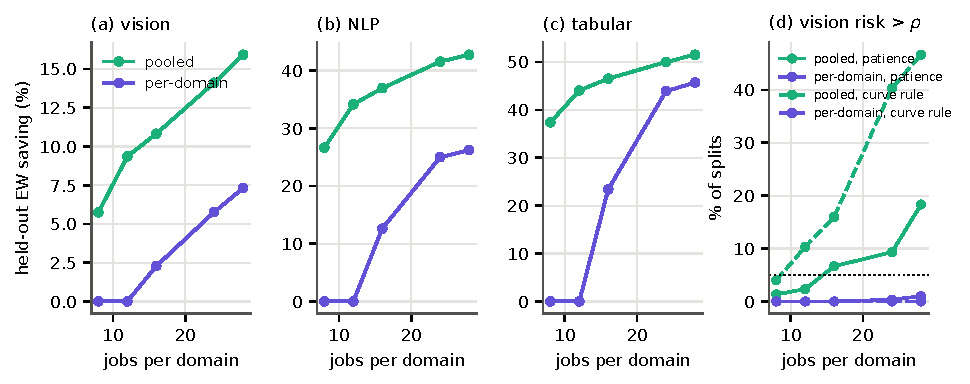
\includegraphics[width=0.9\textwidth]{figures/fig_pool_domain.pdf}
\caption{Pooled against per-domain certification at equal total calibration budget ($\rho=0.20$, $\beta=0.05$, Hoeffding--Bentkus, 259-job pool, 300 random splits per point). (a--c) Energy-weighted saving on held-out jobs of one domain when certifying that domain separately with $n$ jobs (violet) or together with the other two domains, $3n$ jobs in all (aqua). (d) Share of splits whose held-out risk in the vision domain exceeds $\rho$; the dotted line is the 5\% a pooled guarantee permits for the pool, not for a domain.}
\label{fig:pooldomain}
\end{figure*}

\textbf{Cost of failure.} A violation is silent: the stopped model is worse than the full run, and nobody knows unless the run is completed. We therefore charge each violation $c$ full-run energies ($c=1$: the job is re-run to completion; larger $c$ covers diagnosis and re-tuning). With $s$ the energy-weighted saving and $v=\sum_jL_jE_j/\sum_jE_j$ the energy-weighted share of violating runs, the net saving is $s-cv$ and stopping pays only while $c<c^\ast=s/v$. Violations concentrate in the energy-heavy vision jobs, so $v$ is two to three times the job-level risk (Table~\ref{tab:cost}). Pooled out-of-fold, the break-even cost is between 1.4 and 2.9 full-run energies. At $c=1$ the net saving of the framework is 11.5\%, 19.4\% and 14.9\% at $\rho=0.10$, $0.15$ and $0.20$, against 13.2\%, 17.0\% and 18.1\% for calibrated patience under standard certification: the framework's gross advantage of 4 to 7\,pp survives only at $\rho=0.15$ ($+2.4$\,pp) and reverses at the other two ($-1.8$ and $-3.2$\,pp). At $c=0.5$ it stays positive ($+2.5$, $+3.1$, $+1.6$\,pp). The gross savings reported elsewhere in this paper should be read with this in mind: the extra energy the framework saves is, in large part, saved on jobs in which it fails more often.

\begin{table}[t]
\centering
\caption{Cost of failure, pooled out-of-fold over 259 jobs. $s$: energy-weighted saving (\%); $v$: energy-weighted share of violating runs (\%); net: $s-cv$ with each violation charged $c$ full-run energies; $c^\ast=s/v$ is the break-even cost.}
\label{tab:cost}
\footnotesize
\begin{adjustbox}{max width=\columnwidth}
\begin{tabular}{llrrrrr}
\toprule
$\rho$ & Method & $s$ & $v$ & Net, $c{=}1$ & Net, $c{=}3$ & $c^\ast$ \\
\midrule
0.10 & Framework & 27.0 & 15.5 & 11.5 & $-19.6$ & 1.7 \\
 & LTT-HB, patience & 20.2 & 6.9 & 13.2 & $-0.6$ & 2.9 \\
 & LTT-HB, curve rule & 21.9 & 10.8 & 11.1 & $-10.4$ & 2.0 \\
\midrule
0.15 & Framework & 33.3 & 13.9 & 19.4 & $-8.5$ & 2.4 \\
 & LTT-HB, patience & 29.6 & 12.6 & 17.0 & $-8.2$ & 2.3 \\
 & LTT-HB, curve rule & 28.2 & 18.1 & 10.1 & $-26.0$ & 1.6 \\
\midrule
0.20 & Framework & 38.4 & 23.5 & 14.9 & $-32.1$ & 1.6 \\
 & LTT-HB, patience & 32.0 & 13.8 & 18.1 & $-9.6$ & 2.3 \\
 & LTT-HB, curve rule & 33.5 & 23.9 & 9.6 & $-38.3$ & 1.4 \\
\bottomrule
\end{tabular}
\end{adjustbox}
\end{table}

\textbf{The calibrator.} A less conservative guarantee would recover savings, and two lines of work suggest it can: an upper-confidence-bound calibrator and conformal risk control \citep{jazbec2024fastsafe,angelopoulos2024crc}. Both assume a loss that is monotone in the exit parameter; ours is not (Lemma~\ref{lem:monotone}), so we cannot use their guarantees unchanged. We test the part that does not need monotonicity: controlling the \emph{expected} loss, $\mathbb{E}[L_{\hat\theta}]\le\rho$, with the conformal-risk-control criterion $\frac{n}{n+1}\hat R+\frac1{n+1}\le\rho$ in fixed-sequence form (Table~\ref{tab:crc}). It saves more at the same nominal $\rho$ (calibrated patience at $\rho=0.10$: 29.4\% against 20.2\%) but at a higher realised risk (0.082 against 0.045), and it exceeds $\rho$ on held-out data in 4\% to 30\% of splits, as an in-expectation guarantee should. At matched realised risk the saving is the same: CRC at $\rho=0.10$ (risk 0.082) saves 29.4\%, Hoeffding--Bentkus at $\rho=0.15$ (risk 0.085) saves 29.5\%. A less conservative calibrator moves along the same risk--saving frontier; it does not move the frontier.

\begin{table}[t]
\centering
\caption{Calibrators for calibrated patience, pooled out-of-fold over 259 jobs. HB: Hoeffding--Bentkus; betting: betting certificate; CRC: in-expectation conformal-risk-control criterion in fixed-sequence form. EW: energy-weighted saving (\%); ``exceeds'': share of 300 random 70/30 dataset-grouped splits whose held-out risk exceeds $\rho$.}
\label{tab:crc}
\footnotesize
\begin{adjustbox}{max width=\columnwidth}
\begin{tabular}{llrrr}
\toprule
$\rho$ & Calibrator & Risk & EW & Exceeds (\%) \\
\midrule
0.10 & HB & 0.045 & 20.2 & 0 \\
 & Betting & 0.061 & 22.6 & 9 \\
 & CRC & 0.082 & 29.4 & 30 \\
\midrule
0.15 & HB & 0.085 & 29.5 & 0 \\
 & Betting & 0.099 & 31.8 & 0 \\
 & CRC & 0.101 & 32.0 & 4 \\
\midrule
0.20 & HB & 0.101 & 31.9 & 1 \\
 & Betting & 0.118 & 33.6 & 6 \\
 & CRC & 0.184 & 39.1 & 29 \\
\bottomrule
\end{tabular}
\end{adjustbox}
\end{table}

\subsection{RQ8: Does it hold on new fine-tuning data? The confirmatory study}
\label{sec:c1}
\textbf{The rule (pre-registered H1) is not supported.} At a realised risk of at most 0.10, EcoStop-SR saves 33.5\% of energy (energy-weighted) and calibrated patience 43.3\%: a difference of $-9.7$\,pp with a 95\% interval of $[-14.1,+12.1]$ (Table~\ref{tab:c1}). Patience saves more on 24 of the 41 datasets, EcoStop-SR on 13, with 4 ties (sign test $p=0.10$; Fig.~\ref{fig:c1}). At the other risk caps the intervals include zero (point estimates $-0.1$, $+2.3$ and $+2.3$\,pp at 0.05, 0.15 and 0.20). The sign of the primary estimate is fragile: excluding the 14 jobs that barely learn (final test accuracy within 3\,pp of the majority class) gives $+8.3$\,pp ($[-9.8,+16.2]$), thinning EcoStop-SR's $\gamma$ grid gives $-11.2$ ($[-14.9,+11.5]$), and leaving each dataset out in turn gives $-10.2$ to $-8.4$. The pre-registered statistic is the difference between the two rules' best energy-weighted savings among settings whose empirical job-level risk on the 82 jobs is at most 0.10, with that choice repeated in every bootstrap resample. This makes the interval wide and not centred on the estimate: each resample picks the best of many noisy settings, so the bootstrap distribution of the difference has mean $-2.0$\,pp and median $-0.3$\,pp while the point estimate is $-9.7$\,pp. The interval therefore supports only the statement that, allowing for selection noise, no difference can be excluded. Two estimators that do not re-select inside the bootstrap are consistent with each other. Settings fixed on the full sample (EcoStop-SR $\gamma=0.38$, patience $f=0.2$) give $-9.7$\,pp with an interval of $[-15.9,-4.2]$, conditional on a selection made on the same data and so optimistic for both rules. Cross-fitting, in which each rule's setting is chosen on other datasets and scored on held-out ones (100 repeats of 5 dataset-grouped folds, risk cap 0.10), reaches matched realised risks of 0.096 and 0.095 and gives $-5.0$\,pp ($[-11.2,+0.4]$) for EcoStop-SR and $-8.1$\,pp ($[-9.9,-6.5]$) for the paper-gates rule against calibrated patience; this estimator is post hoc. We therefore read C1 as giving no evidence that the curve rule saves more than patience and leaning, at matched risk, towards the opposite. A non-inferiority claim (for instance, not worse by more than 3\,pp) cannot be made, since the lower limits are $-11.2$ and $-14.1$\,pp, and we did not pre-specify a margin and add none after the fact. Under thresholds frozen on the 177 existing jobs, EcoStop-SR saves 10 to 17\,pp less than calibrated patience at the four certified settings (all intervals below zero) and the paper-gates rule 19 to 25\,pp less. With thresholds set on the 35 existing NLP jobs at an empirical risk of at most 0.10, the rules tie ($+0.8$, $[-6.0,+6.6]$) and LC-PFN with SR gates is ahead ($+3.3$, $[+1.0,+5.4]$); at a cap of 0.15 the frozen patience setting realises a risk of 0.20 while the other rules stay below 0.11, which is why they save 12 to 19\,pp less. Per recipe, ELECTRA-small (8 epochs) shows $+9.2$ ($[-3.1,+15.2]$) at risk 0.10 and $+7.4$ ($[+0.1,+10.3]$) at 0.20 for EcoStop-SR, while the 6-layer BERT (12 epochs) shows $-0.5$ and $-14.7$ ($[-16.0,+0.3]$); these are exploratory.

\begin{figure*}[t]
\centering
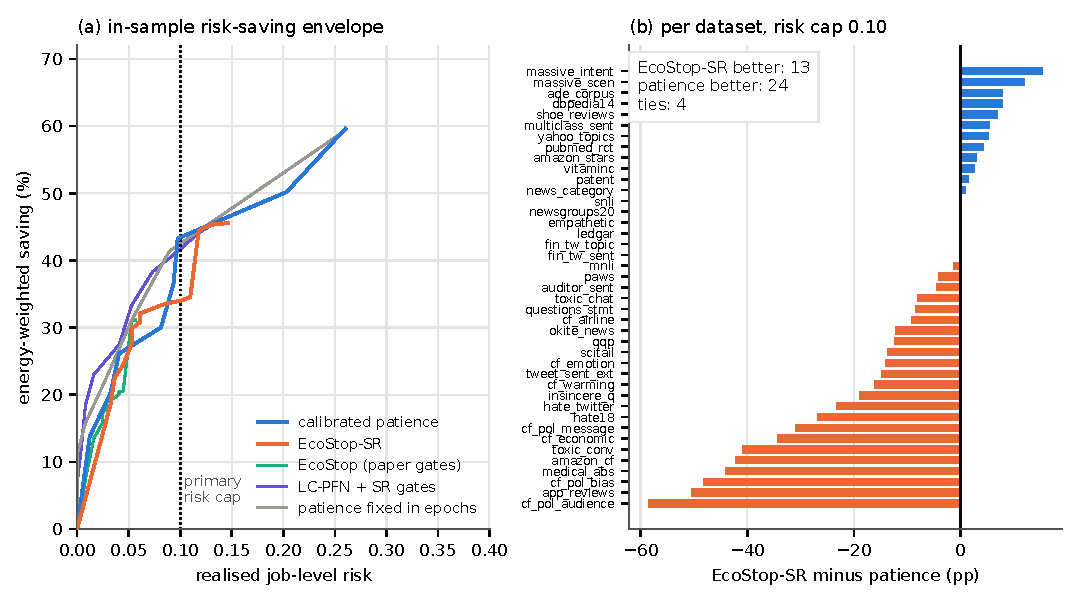
\includegraphics[width=0.92\textwidth]{figures/fig_c1.pdf}
\caption{Confirmatory study C1: 82 fine-tuning jobs on 41 new datasets. (a) In-sample envelope of energy-weighted saving against realised job-level risk for each rule (the best setting at or below each risk); the dotted line is the pre-registered risk cap. (b) Per dataset, energy saved by EcoStop-SR minus calibrated patience at their operating points for risk cap 0.10, as a share of the dataset's energy.}
\label{fig:c1}
\end{figure*}

\begin{table*}[t]
\centering
\caption{Confirmatory study C1 (82 jobs, 41 datasets). Top: the pre-registered rule comparison, EcoStop-SR against calibrated schedule-relative patience; the first row is the primary test. Frozen rows use thresholds calibrated on the 177 existing jobs and applied unchanged. Bottom: the framework (betting certificate, rule selection, scope card) calibrated on the same 177 jobs against standard certification of the best single rule, at the same $\rho$. EW: energy-weighted saving (\%); differences in pp with 95\% bootstrap intervals over datasets. The cross-fitted rows choose each rule's setting on other datasets (realised risk 0.096 for EcoStop-SR, 0.095 for patience, 0.053 for the paper-gates rule).}
\label{tab:c1}
\footnotesize
\begin{adjustbox}{max width=\textwidth}
\begin{tabular}{lrrr}
\toprule
Comparison & EcoStop-SR (EW) & Calibrated patience (EW) & Difference \\
\midrule
\textbf{Primary: risk cap 0.10} & 33.5 & 43.3 & $-9.7$ $[-14.1,+12.1]$ \\
Risk cap 0.05 & 26.0 & 26.1 & $-0.1$ $[-10.7,+11.8]$ \\
Risk cap 0.15 & 45.5 & 43.3 & $+2.3$ $[-8.7,+3.5]$ \\
Risk cap 0.20 & 45.5 & 43.3 & $+2.3$ $[-12.3,+3.7]$ \\
Cross-fitted, risk cap 0.10 (post hoc) & 34.2 & 39.2 & $-5.0$ $[-11.2,+0.4]$ \\
Cross-fitted, paper-gates rule (post hoc) & 31.1 & 39.2 & $-8.1$ $[-9.9,-6.5]$ \\
Frozen, Hoeffding--Bentkus $\rho=0.15$ & 24.5 & 36.5 & $-12.1$ $[-18.7,-6.2]$ \\
Frozen, betting $\rho=0.15$ & 26.0 & 43.3 & $-17.3$ $[-23.6,-11.7]$ \\
Frozen, Hoeffding--Bentkus $\rho=0.20$ & 32.1 & 43.3 & $-11.2$ $[-17.7,-5.5]$ \\
Frozen, betting $\rho=0.20$ & 33.6 & 43.3 & $-9.7$ $[-16.1,-4.1]$ \\
\midrule
 & Framework: risk (EW) & Best single LTT-HB (EW) & Difference \\
\midrule
$\rho=0.10$ & 0.041 (20.4) & 0.081 (30.0) & $-9.6$ $[-15.4,-4.4]$ \\
$\rho=0.15$ & 0.098 (43.3) & 0.093 (36.5) & $+6.7$ $[+5.9,+7.7]$ \\
$\rho=0.20$ & \textbf{0.203} (50.2) & 0.098 (43.3) & $+6.9$ $[+5.7,+8.1]$ \\
\bottomrule
\end{tabular}
\end{adjustbox}
\end{table*}

\textbf{The framework (held-out check).} Calibrated on the 177 existing jobs only and applied unchanged, the framework's realised risk on C1 is 0.041, 0.098 and 0.203 at $\rho=0.10$, $0.15$ and $0.20$ (Table~\ref{tab:c1}, bottom). By the criterion we set (risk at most $\rho$ at all three targets) the validity claim is not met at $\rho=0.20$, by 0.003. That margin is well inside the sampling error of 82 jobs, and the guarantee is probabilistic over calibration sets and about population risk, which one realisation cannot test; we nevertheless report it as a miss. In efficiency, the framework saves 6.7 and 6.9\,pp more than the best single-rule standard certificate at $\rho=0.15$ and $0.20$ and 9.6\,pp less at $\rho=0.10$; these are gains at the same certified target and not at the same realised risk (0.098 against 0.093 at $\rho=0.15$, and 0.203 against 0.098 at $\rho=0.20$, so the larger saving at $\rho=0.20$ is bought with twice the realised risk). Their intervals are about 2\,pp wide, against 26\,pp for the rule comparison, because the settings were frozen on the 177 earlier jobs and only the 82 jobs are resampled, whereas the rule comparison also resamples the choice of setting. At $\rho=0.10$, where selection chose the curve rule at a conservative setting. The gain is the betting bound permitting calibrated patience one setting more aggressive than the Hoeffding--Bentkus bound does (setting 5 against 4 at $\rho=0.15$); the betting certificate on patience alone gives the same savings. Rule selection and the scope card are not exercised, since C1 is a single domain and every job is in scope. The size of the gain depends on how much calibration data patience has: with 117 NLP jobs in the pooled analysis the margin over standard certification in NLP shrinks to $+0.9$ and $-0.3$\,pp (Table~\ref{tab:regime}).

\subsection{RQ9: Does validating more often pay for itself in small-language-model fine-tuning?}
\label{sec:slm}
Fine-tuning holds most of the remaining headroom, and small language models are fine-tuned with evaluation every few hundred steps, not every epoch. A natural extension of the framework is therefore to take stopping decisions at finer granularity and certify them. We ran a pilot to test whether finer decisions pay for the extra validation passes, with a gate set in advance for each question (energy of a validation pass, headroom, net oracle saving).

\textbf{Pilot.} Qwen2.5-0.5B-Instruct was fine-tuned with LoRA (rank 16, learning rate $2\times10^{-4}$, three epochs, batch 16, 3{,}840 training, 500 validation and up to 1{,}000 test examples) on classification tasks scored by the log-likelihood of a label letter after the prompt. Validation and test accuracy were logged every eighth of an epoch (24 points per run), with NVML energy metered separately for training, validation passes and the audit test passes; the test passes are excluded from deployed energy. Granularities of an eighth, a quarter, a half and one epoch are obtained by keeping every $g$-th point. Four short-text tasks from the C1 pool, reusing its splits (news topics, textual entailment, airline sentiment, paraphrase), completed with two seeds each. Two long-text tasks (medical abstracts, review ratings) were planned; the pilot was stopped during the first of them, after 11 of 24 points, once it was clear that the first gate would fail by a wider margin there.

\begin{table*}[t]
\centering
\caption{Small-language-model pilot (Qwen2.5-0.5B, LoRA; 8 completed runs on four short-text tasks). Energy is net of validation passes and relative to the epoch-level full run. ``Oracle'': hindsight stop at the earliest point whose test accuracy is within 0.5\,pp of the final one. ``Validation share'': validation passes as a share of deployed energy. Patience is counted in evaluation points; the setting shown is the one with a violation rate near 0.12 where one exists.}
\label{tab:slm}
\footnotesize
\begin{adjustbox}{max width=\textwidth}
\begin{tabular}{lrrrrr}
\toprule
Granularity & Oracle net saving (\%) & Validation share (\%) & Patience (points) & Violation rate & Net saving (\%) \\
\midrule
1 epoch & 48.8 & 3.7 & 1 & 0.12 & 16.9 \\
1/2 epoch & 53.3 & 7.1 & 2 & 0.12 & 17.9 \\
1/4 epoch & 47.5 & 13.4 & 4 & 0.12 & 10.5 \\
1/8 epoch & 62.6 & 23.5 & 8 & 0.25 & 5.8 \\
\bottomrule
\end{tabular}
\end{adjustbox}
\end{table*}

\textbf{Result.} Headroom exists: the oracle stops at a median of 50\% of the training steps at quarter-epoch granularity (gate: at most 60\%, passed) and a deployed epoch-level run takes 2.4\,min (gate: at most 15\,min, passed). Validation is not free. A pass over 500 validation examples costs about a third of the training between two eighth-epoch points on short text, so validation takes 13.4\% of deployed energy at quarter-epoch granularity (gate: at most 10\%, failed) and 23.5\% at an eighth. On long text it is worse: in the partial medical-abstract run a validation pass cost 0.75 of a training chunk, 30\% of deployed energy at quarter-epoch granularity and 12.6\% even at epoch level. The net oracle saving at quarter-epoch granularity is 1.3\,pp \emph{below} the epoch-level one (gate: at least 5\,pp above, failed); the higher oracle value at an eighth of an epoch (62.6\%) is the best of 24 noisy points and is not realised by any rule. Patience counted in evaluation points does not exploit finer granularity: at a violation rate near 0.12, epoch-level patience of one point saves 16.9\% net, half-epoch patience 17.9\% and quarter-epoch patience 10.5\%, and the eighth-epoch grid has no setting below 0.25 that saves energy. Detecting the plateau on validation loss, which is smoother, did not change this (at quarter-epoch granularity with patience 4 the violation rate rose from 0.12 to 0.25).

\textbf{Reading.} With validation sets of this size, finer decisions do not repay their own energy, and noise in the validation signal makes patience fire at the wrong place. We therefore did not proceed to a calibration or confirmatory study, and the framework claims of this paper do not extend to decoder language-model fine-tuning. The pilot is small (8 complete runs, one model, four tasks) and says nothing about much larger validation sets, sub-sampled validation, or other models; it rules out one tempting route, not the setting.

\subsection{RQ10: Does energy carry information beyond epoch count?}
\label{sec:rq6}
All stopping rules here decide from validation accuracy; energy enters only in how savings are scored. Whether that distinction matters depends on whether per-epoch cost is constant. Under fixed-resolution training, an energy oracle and an epoch oracle choose almost the same stopping epoch (mean absolute difference 0.01--0.42 epochs across four pilot cells; Fig.~\ref{fig:rq0-cdf}). Under progressive image resizing (16 to 32\,px in four phases, CIFAR-10, three seeds), where later epochs cost far more (Fig.~\ref{fig:progressive-mechanism}), they disagree: 0.66 epochs from an epoch oracle and 0.53 from a wall-clock oracle, with agreement at zero difference falling from about 97\% to about 80\%.

We tested a second variable-cost regime, layer freeze/thaw: ResNet-9 with the first four stages frozen for epochs 0--11 (backward then stops at the third stage and per-epoch energy steps up at the thaw), on six datasets with three seeds. The hindsight oracle saves 30.3\% of energy for 27.9\% of epochs, a gap of $+2.4$\,pp; the same recipe without freezing shows $-0.1$\,pp over the same six datasets. At the same stopping epochs, energy saved exceeds epochs saved by 0.5--2.1\,pp at $\rho=0.20$, more for the rules that stop earlier (Table~\ref{tab:b2}). Energy therefore carries information beyond epoch count only when cost is nonstationary, and only a few points in these regimes.

The same regime stresses the rules. At $\rho=0.20$ every frozen pooled threshold breaches its target on these six jobs (risk 0.22--0.44): after thaw the accuracy jumps from a plateau, the pattern that defeated step-decay and one-cycle schedules in \S\ref{sec:b1}. At $\rho=0.15$ all rules stay within target (0.06--0.11). With 18 runs on six datasets these figures are indicative, not conclusive. We did not build an energy-aware stopping rule; this section shows only that the scoring of savings, not the stopping decision, is where energy matters under the cost patterns tested.

\begin{figure*}[t]
\centering
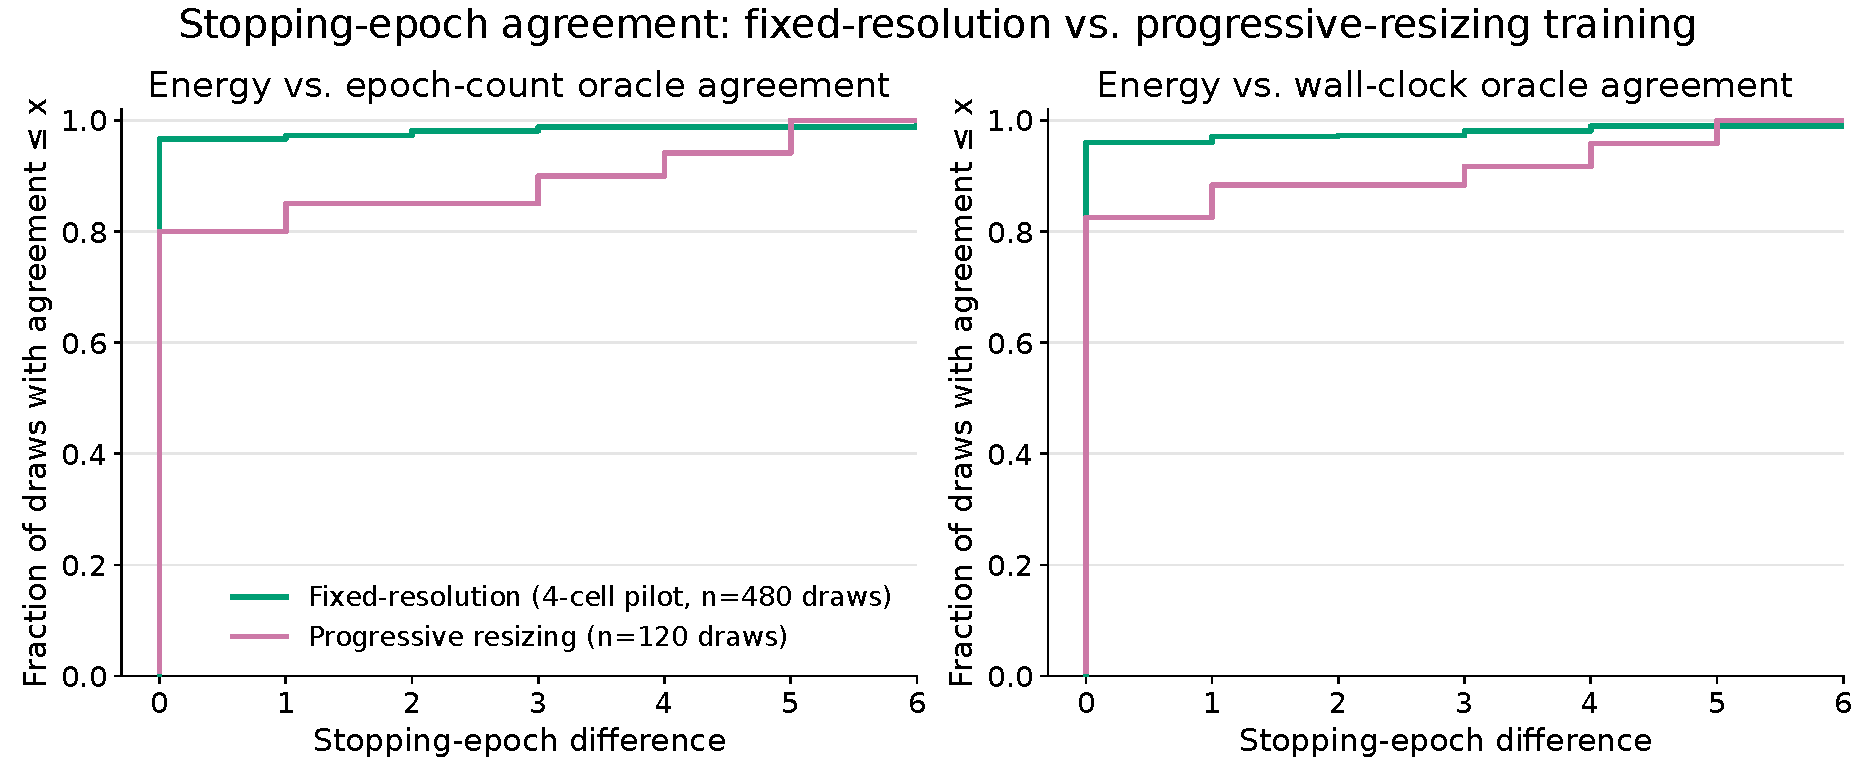
\includegraphics[width=0.62\textwidth]{figures/figure1.pdf}
\caption{Energy versus epoch/time-count agreement: empirical CDFs of the stopping-epoch difference between an energy oracle and an epoch- or wall-clock-count oracle, fixed-resolution pilot versus progressive-resizing runs.}
\label{fig:rq0-cdf}
\end{figure*}

\begin{figure*}[t]
\centering
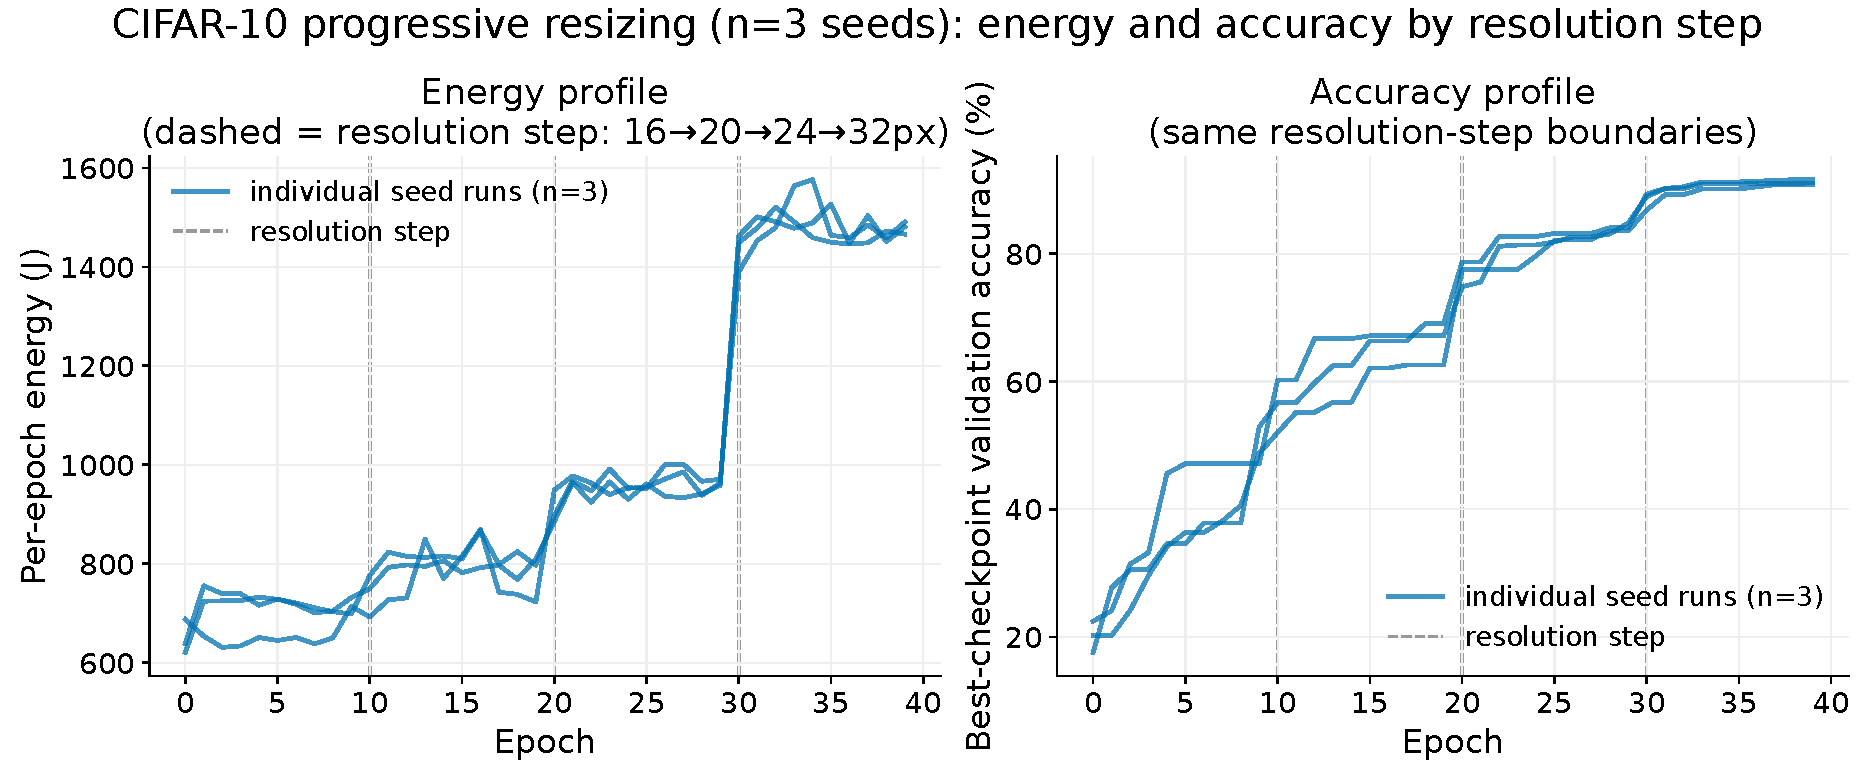
\includegraphics[width=0.62\textwidth]{figures/figure2.pdf}
\caption{Mechanism behind the divergence under progressive resizing: per-epoch energy jumps at each resolution step (CIFAR-10), so epoch count and energy stop tracking each other.}
\label{fig:progressive-mechanism}
\end{figure*}

\begin{table}[t]
\centering
\caption{Frozen pooled thresholds on the layer freeze/thaw regime (6 datasets, 18 runs). ``Epochs saved'' and ``energy saved'' are per-job means at the same stopping epochs; EW is the energy-weighted saving.}
\label{tab:b2}
\footnotesize
\begin{adjustbox}{max width=\columnwidth}
\begin{tabular}{p{3.0cm}rrrr}
\toprule
Rule & Risk & \shortstack{Epochs\\saved (\%)} & \shortstack{Energy\\saved (\%)} & \shortstack{EW\\(\%)} \\
\midrule
\multicolumn{5}{l}{\emph{Frozen target $\rho=0.15$}}\\
EcoStop & 0.111 & 13.8 & 15.0 & 20.3 \\
Patience, $p=\lceil fT\rfloor$, min-$\delta$ & 0.056 & 6.8 & 7.2 & 6.4 \\
Patience, $p=\lceil fT\rfloor$ & 0.056 & 3.2 & 3.2 & 1.0 \\
Patience, fixed $p$ & 0.056 & 3.2 & 3.2 & 1.0 \\
\midrule
\multicolumn{5}{l}{\emph{Frozen target $\rho=0.20$}}\\
EcoStop & 0.444 & 32.2 & 34.3 & 37.4 \\
Patience, $p=\lceil fT\rfloor$, min-$\delta$ & 0.444 & 28.9 & 30.8 & 30.7 \\
Patience, $p=\lceil fT\rfloor$ & 0.389 & 23.3 & 24.6 & 22.4 \\
Patience, fixed $p$ & 0.222 & 12.5 & 13.0 & 8.6 \\
\bottomrule
\end{tabular}
\end{adjustbox}
\end{table}

\subsection{RQ11: How reliable is the energy measurement?}
\label{sec:rq6b}
\textbf{Idle power and sensor.} Board power at rest is 15.3\,W (60\,s average). Subtracting idle power times duration from every run's energy changes the corpus energy-weighted saving from 32.0\% to 32.3\% at the same stopping decisions, although idle power is 16.1\% of total energy; the savings are therefore insensitive to the baseline. The NVML power value updates only about every 0.5\,s (median interval 0.500\,s, 90th percentile 0.516\,s) regardless of how often it is polled. Vision and NLP epochs last tens of seconds and contain dozens of sensor updates, but tabular epochs (tens of milliseconds to under a second) fall below the update interval: their per-epoch energy is close to duration times a held power value, so percentage savings on tabular jobs are in effect time savings. The energy-weighted metrics, to which tabular jobs contribute almost nothing (a mean of 82\,J per run), are unaffected.

\textbf{Repeatability.} Five identical runs of one job (SEMEION, ResNet-9, 40 epochs, same seed) consumed $9.40$\,kJ on average with a coefficient of variation of 1.95\% (range $9.21$--$9.70$\,kJ); duration varied by 4.2\%. Savings are ratios within a run, so this variation cancels to first order. The same repeats also differ in accuracy (best validation accuracy 67.9--82.4\%), which reflects non-deterministic GPU training on a very small dataset, not measurement noise; it is one reason we treat seeds as nested within jobs.

\section{Discussion}
\label{sec:discussion}

\textbf{What the results imply.} Four findings hold across the development, fresh and confirmatory sets. First, certification is where most of the benefit lies: calibrated against a stated risk, even plain patience saves 30 to 32\% of energy (energy-weighted, pooled out-of-fold at $\rho=0.15$--$0.20$) where the patience values in use either break the tolerance or save almost nothing. Second, a schedule-relative safeguard, not the learning-curve model, determines whether a rule works: at matched certified risk the curve score adds nothing and raises vision risk. Third, a guarantee that holds within each domain is expensive. Pooling is what makes certification cheap, and it does so by letting the domain with the most energy and the hardest curves exceed its target while the pool stays within it. Fourth, the framework's gain over standard certification (3.8 to 6.8\,pp, pooled out-of-fold) is regime-dependent, comes with a higher realised risk, and is largely consumed by violations in the heaviest jobs once each is charged a re-run (\S\ref{sec:cost}). The practical recommendation is therefore modest and conditional: for fine-tuning, use a patience proportional to the schedule length with a small minimum improvement, calibrate it with the procedure of \S\ref{sec:problem}, and do not rely on a fixed patience in epochs; for long annealed runs, certify and select among rules per domain and decide, from the cost of a failed run, whether the extra saving is worth the extra risk. When the training length is unknown, schedule-relative patience is unavailable and the curve rule did better (an exploratory result, \S\ref{sec:ablation}).

Combining detectors did not help. We tried four consensus rules fixed in advance (stop only when the curve rule and patience agree, when the curve rule and LC-PFN agree, when any two of the three agree, and when all three agree), each certified like a single rule. On the development jobs none beat calibrated patience at matched risk (differences between $-4.0$ and $+2.8$\,pp), and on the fresh jobs the only intervals excluding zero were one against consensus and two at an unmatched realised risk.

\textbf{An exploratory negative result: certified early cooldown.} Stopping on a plateau forfeits the annealing gain, so we asked whether the decision should be ``start the cooldown'' instead of ``stop'': train at a stable learning rate and, when a trigger fires, decay the learning rate to zero over eight epochs and stop. On six datasets and two seeds (ResNet-9, 12 runs) a cooldown from an early checkpoint matched the full run within 0.5\,pp for 10 of 12 runs, and an adaptive trigger based on EcoStop's score saved 28\% of the epochs at no more than 10\% violation, where no fixed trigger epoch saved anything. Against the right baseline, however, the advantage disappears: stopping a recipe-matched cosine run with the same rule saved 25\% at the same violation level (and 32\% at 20\%). An earlier comparison against the cosine recipe of our corpus had suggested a large gain, but that recipe was up to 8\,pp worse on harder datasets, so the gain was a baseline artefact. We did not pursue a larger study. The episode illustrates why every comparison in this paper is made against a baseline of equal quality at matched certified risk.

\textbf{Limitations.}
(i) \emph{Regime and scope.} The regime map was found after the pre-registered confirmatory study failed to favour the curve rule; it is exploratory. Its subgroup intervals are not corrected for the number of subgroups examined. Schedule is confounded with domain, model and data scale, so we cannot say that annealing itself is the cause. We make no claim for decoder language-model fine-tuning or for large-scale pretraining: our small-language-model evidence is a pilot on one 0.5B model (\S\ref{sec:slm}).
(ii) \emph{The guarantee is pooled.} It holds on the declared mix of domains, not within each domain: vision reached a realised risk of 0.30 at $\rho=0.20$ under the framework (0.18 under patience), and 0.31 on the cosine-annealed ResNet-9 jobs alone, and per-domain certification saves 6 to 18\,pp less at 28 jobs per domain and certifies nothing below 16 jobs per domain at $\rho=0.15$ (\S\ref{sec:cost}). The framework's vision gains are not matched in risk.
(iii) \emph{Confirmatory evidence is partial.} In the confirmatory study the curve rule did not beat patience (an interval of $[-14.1,+12.1]$ that does not rule out a small benefit), the framework check missed its validity criterion at $\rho=0.20$ by 0.003, lost at $\rho=0.10$, and could not exercise rule selection or the scope card, since all its jobs are in one domain and in scope (both are evaluated on the development, fresh and pooled data, \S\ref{sec:ext}, \S\ref{sec:b1} and \S\ref{sec:regime}). The pre-registered statistic is wide because it re-selects the setting in every resample; the matched-risk cross-fitted estimate ($-5.0$\,pp, $[-11.2,+0.4]$) is post hoc. The pooled framework result, which is strongest, is out-of-fold on data the authors had seen.
(iv) \emph{Scale and hardware.} Jobs are benchmark-sized (the corpus consumed 5.2\,kWh before C1 and policies avoid about a third of it when energy-weighted), and all runs use one laptop GPU on a workstation that was shared with unrelated work at times, which adds to a run's board energy; the C1 runs also met suspensions, quarantined runs and power-offs (\S\ref{sec:c1setup}). Savings are ratios within a run, which limits but does not remove the effect, and NVML reports board power, not system power (\S\ref{sec:rq6b}). The tabular models are small MLPs, which are not state of the art for tabular data \citep{grinsztajn2022tabular}.
(v) \emph{Population assumption and tolerance.} The guarantee (Assumption~\ref{ass:iid}) concerns independent jobs drawn from the declared mix of architectures, recipes and schedule lengths; \S\ref{sec:b1} tests a deliberate shift and locates its boundary: schedule families absent from calibration (step decay, one-cycle) and discontinuous regimes such as layer thawing (\S\ref{sec:rq6}) break the guarantee at $\rho=0.20$. We fix $\epsilon=0.5$\,pp; other tolerances are covered by the sensitivity analysis only.
(vi) \emph{Design leakage.} The constants of the rules were tuned on the development corpus, which is why the fresh and confirmatory sets were frozen first; the scope descriptors, by contrast, were chosen after we saw which fresh jobs failed, so the abstention result needs a confirmatory set of its own.
(vii) \emph{Cost of failure and seed noise.} The cost model of \S\ref{sec:cost} charges every violation the same multiple of the job's energy and treats violations as detectable; in practice they are silent and their cost depends on the application. Seed-to-seed variation exceeds the tolerance in two thirds of the jobs (\S\ref{sec:ablation}), and part of every vision risk is test-set noise that no stopping rule can remove.

\section{Conclusion}
\label{sec:conclusion}
Early stopping saves energy only to the extent that its accuracy risk is controlled, and rules can be compared fairly only at matched risk. Under that comparison, rules with a schedule-relative safeguard are interchangeable on average, the learning-curve score adds nothing, and patience fixed in epochs is not competitive. A guarantee that holds per domain is expensive, and the cheap pooled guarantee lets the heaviest domain exceed its target. A framework of a betting certificate, certified rule selection and a scope card saves 3.8 to 6.8\,pp more than standard certification at the same certified target, pooled out-of-fold over 259 jobs, at a higher realised risk and with a lead that, net of the cost of failed runs, survives at one of three targets. A pre-registered confirmatory study of 82 jobs on 41 new datasets found no advantage for the curve rule. The certificate should be re-issued, or made to abstain, when the schedule family changes. We release the logs, the frozen protocols and the analysis code with this paper.

\section*{Declaration of competing interest}
The authors declare that they have no known competing financial interests or personal relationships that could have appeared to influence the work reported in this paper.

\section*{Data and code availability}
All data, protocols and code are publicly available at \url{https://github.com/habibullahmanzoor/ecostop}. The repository contains EcoStop-Bench (923 metered runs, loader and matched-risk protocol), the frozen protocols with their SHA-256 hashes (\texttt{b1\_protocol.json}, \texttt{c1\_protocol.json}, the C1 dataset manifest and analysis plans), a log of every protocol deviation, the raw per-run logs of the development, fresh and confirmatory studies including the quarantined runs and the GPU health logs, all analysis code and result tables, and a SHA-256 manifest. Every number in this paper can be recomputed from it on a CPU. The exact version used in this paper is tagged 	exttt{v1.0}.

\section*{Declaration of generative AI and AI-assisted technologies in the writing process}
During the preparation and revision of this work, the authors used AI assistants, including Claude (Anthropic) and ChatGPT (OpenAI), to assist with drafting, restructuring, language revision, internal-consistency checking, and analysis and figure code preparation. The authors reviewed and edited the resulting content as needed and take full responsibility for the content of the article.

\bibliographystyle{elsarticle-num-names}
\bibliography{references}

\end{document}
